% Options for packages loaded elsewhere
\PassOptionsToPackage{unicode}{hyperref}
\PassOptionsToPackage{hyphens}{url}
\PassOptionsToPackage{dvipsnames,svgnames,x11names}{xcolor}
\documentclass[
  10pt,
]{article}
\usepackage{xcolor}
\usepackage[margin=20mm]{geometry}
\usepackage{amsmath,amssymb}
\setcounter{secnumdepth}{-\maxdimen} % remove section numbering
\usepackage{iftex}
\ifPDFTeX
  \usepackage[T1]{fontenc}
  \usepackage[utf8]{inputenc}
  \usepackage{textcomp} % provide euro and other symbols
\else % if luatex or xetex
  \usepackage{unicode-math} % this also loads fontspec
  \defaultfontfeatures{Scale=MatchLowercase}
  \defaultfontfeatures[\rmfamily]{Ligatures=TeX,Scale=1}
\fi
\usepackage{lmodern}
\ifPDFTeX\else
  % xetex/luatex font selection
    \setmainfont[]{Times New Roman}
    \setmonofont[]{Menlo}
\fi
% Use upquote if available, for straight quotes in verbatim environments
\IfFileExists{upquote.sty}{\usepackage{upquote}}{}
\IfFileExists{microtype.sty}{% use microtype if available
  \usepackage[]{microtype}
  \UseMicrotypeSet[protrusion]{basicmath} % disable protrusion for tt fonts
}{}
\makeatletter
\@ifundefined{KOMAClassName}{% if non-KOMA class
  \IfFileExists{parskip.sty}{%
    \usepackage{parskip}
  }{% else
    \setlength{\parindent}{0pt}
    \setlength{\parskip}{6pt plus 2pt minus 1pt}}
}{% if KOMA class
  \KOMAoptions{parskip=half}}
\makeatother
\usepackage{longtable,booktabs,array}
\usepackage{calc} % for calculating minipage widths
% Correct order of tables after \paragraph or \subparagraph
\usepackage{etoolbox}
\makeatletter
\patchcmd\longtable{\par}{\if@noskipsec\mbox{}\fi\par}{}{}
\makeatother
% Allow footnotes in longtable head/foot
\IfFileExists{footnotehyper.sty}{\usepackage{footnotehyper}}{\usepackage{footnote}}
\makesavenoteenv{longtable}
\usepackage{graphicx}
\makeatletter
\newsavebox\pandoc@box
\newcommand*\pandocbounded[1]{% scales image to fit in text height/width
  \sbox\pandoc@box{#1}%
  \Gscale@div\@tempa{\textheight}{\dimexpr\ht\pandoc@box+\dp\pandoc@box\relax}%
  \Gscale@div\@tempb{\linewidth}{\wd\pandoc@box}%
  \ifdim\@tempb\p@<\@tempa\p@\let\@tempa\@tempb\fi% select the smaller of both
  \ifdim\@tempa\p@<\p@\scalebox{\@tempa}{\usebox\pandoc@box}%
  \else\usebox{\pandoc@box}%
  \fi%
}
% Set default figure placement to htbp
\def\fps@figure{htbp}
\makeatother
\setlength{\emergencystretch}{3em} % prevent overfull lines
\providecommand{\tightlist}{%
  \setlength{\itemsep}{0pt}\setlength{\parskip}{0pt}}

\usepackage{fancyhdr}
\pagestyle{fancy}
\fancyhf{}
\fancyhead[L]{\small\textcolor[gray]{0.4}{SimPT60: Time-Series Power-Flow Dataset}}
\fancyhead[R]{\small\textcolor[gray]{0.4}{September 2026}}
\fancyfoot[C]{\small\thepage}
\renewcommand{\headrulewidth}{0.4pt}
\renewcommand{\footrulewidth}{0pt}

\usepackage{setspace}
\setstretch{1.16}
\setlength{\emergencystretch}{3em}
\setlength{\parskip}{0.4em plus 0.1em minus 0.1em}
\setlength{\parindent}{0pt}
% Native XeTeX line breaking works without a separate xeCJK installation.
\XeTeXlinebreaklocale "zh"
\XeTeXlinebreakskip = 0pt plus 1pt
% Use the page-builder-aware package, including at a natural page break.
\usepackage{needspace}
\newcommand{\PTneedspace}[1]{\Needspace{#1}}

\usepackage{titlesec}
\titleformat{\section}{\Large\bfseries}{\thesection}{0.8em}{}
\titleformat{\subsection}{\large\bfseries}{\thesubsection}{0.8em}{}
\titleformat{\subsubsection}{\normalsize\bfseries}{\thesubsubsection}{0.8em}{}
\titlespacing*{\section}{0pt}{14pt plus 2pt minus 2pt}{6pt plus 1pt minus 1pt}
\titlespacing*{\subsection}{0pt}{10pt plus 2pt minus 2pt}{4pt plus 1pt minus 1pt}
\titlespacing*{\subsubsection}{0pt}{8pt plus 1pt minus 1pt}{3pt plus 1pt minus 1pt}

\usepackage{booktabs}
\usepackage{array}
\usepackage{colortbl}

% Ensure inline graphics are centered
\let\origpandocbounded\pandocbounded
\renewcommand*\pandocbounded[1]{%
  \begin{center}%
  \origpandocbounded{#1}%
  \end{center}%
}
\usepackage{bookmark}
\IfFileExists{xurl.sty}{\usepackage{xurl}}{} % add URL line breaks if available
\urlstyle{same}
\hypersetup{
  pdftitle={SimPT60: A Traceable Time-Series Power-Flow Dataset for Portugal's High-Voltage Grid},
  colorlinks=true,
  linkcolor={blue},
  filecolor={Maroon},
  citecolor={Blue},
  urlcolor={blue},
  pdfcreator={LaTeX via pandoc}}

\title{SimPT60: A Traceable Time-Series Power-Flow Dataset for
Portugal's High-Voltage Grid}
\author{}
\date{September 2026}

\begin{document}
\maketitle
\begin{abstract}
Publicly accessible power-system data are commonly fragmented across
network structure, equipment attributes, and operating records, which
limits their direct use in continuous power-flow analysis and method
comparison. We present SimPT60, a research dataset reconstructed from
multiple public sources for the continental Portuguese 60--400 kV grid
and the Portugal--Spain interconnection boundary. SimPT60 organizes the
static network, operating time series, and alternating-current
power-flow results in a unified data framework. It provides continuous
15-minute operating cases, source-level provenance, and validation
products for assessing model consistency. The dataset supports
time-series power-flow studies, scenario comparison, relative-risk
screening, and testing of grid-analysis algorithms. Its research utility
is demonstrated using E-REDES public datasets that were withheld from
nodal-power construction, parameter-sensitivity experiments, and N−1
contingency screening. SimPT60 is a public-data-derived research model
and has not been validated as an operator network model at equipment
level.

\textbf{Keywords:} power-system dataset; Portugal; public data; grid
reconstruction; power flow; time series; provenance; cross-source
validation
\end{abstract}

\section{1. Introduction}\label{introduction}

Power-flow simulation underpins many studies of grid operation,
planning, and risk, and requires data that describe network topology,
equipment attributes, and operating conditions
(\hyperref[ref-Thurner2018]{Thurner et al., 2018}). As research moves
from individual snapshots to time-series analysis, a static network must
also be linked to continuous load, generation, and other operating
records (\hyperref[ref-Horsch2018]{Hörsch et al., 2018};
\hyperref[ref-Meinecke2020]{Meinecke et al., 2020}).

Several public resources already provide reusable grid models and
benchmark datasets. PyPSA-Eur supplies a transmission-network model for
European energy-system optimization and operational studies
(\hyperref[ref-Horsch2018]{Hörsch et al., 2018}). Recent open-data
reconstruction work has expanded the geographic representation of the
European high-voltage grid (\hyperref[ref-Xiong2025]{Xiong et al.,
2025}). SimBench provides representative networks across several voltage
levels together with annual load and generation profiles
(\hyperref[ref-Meinecke2020]{Meinecke et al., 2020}). These resources
support system optimization, network reconstruction, and method
comparison, respectively, and provide an important basis for open
power-system research.

\subsection{1.1 Motivation}\label{motivation}

Portugal's National Energy and Climate Plan identifies renewable
generation, storage, electrification, and cross-border interconnection
as central elements of the energy transition
(\hyperref[ref-DGEGPNEC2030Revision2024]{DGEG, 2024}). These
developments alter the scale and spatial distribution of generation and
demand and therefore affect line flows, bus voltages, and system risk.
Studying the time-varying behavior of the Portuguese grid consequently
requires a data foundation that represents both network structure and
continuous operating conditions.

The relevant public records are distributed across E-REDES, Redes
Energéticas Nacionais (REN), the Direção-Geral de Energia e Geologia
(DGEG), the Entidade Reguladora dos Serviços Energéticos (ERSE), and
open geospatial platforms (\hyperref[ref-EREDESRND2026]{E-REDES,
n.d.-f}; \hyperref[ref-RENDataHub2026]{REN, n.d.};
\hyperref[ref-DGEGGeo2026]{DGEG, n.d.};
\hyperref[ref-ERSEPDIRT2024]{REN, 2024};
\hyperref[ref-OSM2026]{OpenStreetMap contributors, n.d.}). Their spatial
coverage, temporal resolution, identifiers, and field definitions
differ. Using them in a common power-flow model requires topology
reconstruction, completion of electrical parameters, asset-to-bus
mapping, temporal alignment, and allocation of aggregate power to nodes.

Existing resources also have different modelling objectives and scopes.
European-scale models primarily address cross-regional system studies
(\hyperref[ref-Horsch2018]{Hörsch et al., 2018}); open high-voltage
reconstructions focus mainly on AC networks at 220 kV and above
(\hyperref[ref-Xiong2025]{Xiong et al., 2025}); and representative
benchmarks do not describe the geographic Portuguese grid
(\hyperref[ref-Meinecke2020]{Meinecke et al., 2020}). A public research
resource that combines the continental Portuguese 60--400 kV network,
15-minute operating time series, solvable power-flow cases, and explicit
provenance has therefore remained unavailable.

This study develops a traceable, computationally usable Portuguese
high-voltage grid dataset with continuous time-indexed cases for
power-flow analysis, grid-risk screening, scenario comparison, and
method testing.

\subsection{1.2 Introducing SimPT60}\label{introducing-simpt60}

SimPT60 reconstructs the continental Portuguese high-voltage grid from
multiple public sources. It covers the 60, 130, 150, 220, and 400 kV
networks and retains the boundary nodes required to represent
Portugal--Spain interconnections. Raw sources, the static network,
time-series inputs, power-flow results, and validation records are
stored in linked layers so that users can trace key fields to their
source and processing rule.

The main contribution is a versioned data product that links a traceable
public-data reconstruction of the continental Portuguese 60--400 kV grid
to 31,492 consecutive and reproducible 15-minute AC power-flow states.
Raw records, derived objects, and validation results remain separate but
connected. Table 1 summarizes the scope, principal products, and
interpretation boundaries; Section 4.7 states the limitations.

\PTneedspace{288pt}

\textbf{Table 1---Scope and data products of SimPT60.}

\begin{longtable}[]{@{}
  >{\raggedright\arraybackslash}p{(\linewidth - 4\tabcolsep) * \real{0.3333}}
  >{\raggedright\arraybackslash}p{(\linewidth - 4\tabcolsep) * \real{0.3333}}
  >{\raggedright\arraybackslash}p{(\linewidth - 4\tabcolsep) * \real{0.3333}}@{}}
\toprule\noalign{}
\begin{minipage}[b]{\linewidth}\raggedright
Dimension
\end{minipage} & \begin{minipage}[b]{\linewidth}\raggedright
Scope or product
\end{minipage} & \begin{minipage}[b]{\linewidth}\raggedright
Interpretation boundary
\end{minipage} \\
\midrule\noalign{}
\endhead
\bottomrule\noalign{}
\endlastfoot
Geography & Continental Portugal and Portugal--Spain boundary endpoints
& Excludes islands and distribution networks below 60 kV \\
Voltage & 60, 130, 150, 220, and 400 kV & Reconstructed from multiple
public sources \\
Time & 2025-05-01 to 2026-03-24; 15 min & Europe/Lisbon civil days;
aligned in Coordinated Universal Time (UTC) \\
Static network & Buses, lines, transformers, assets, and geometry &
Public connection evidence and engineering proxies coexist \\
Operating cases & 31,492 steady-state AC power-flow cases & Computed
model states, not equipment telemetry \\
Distribution and provenance & Main database, 11 monthly databases,
raw-record locators, and source hashes & Source licensing and release
snapshots are managed separately \\
Validation and application & External temporal/spatial comparisons,
perturbation tests, stress scenarios, and N−1 & Aggregate consistency
does not establish equipment-level truth \\
\end{longtable}

\textbf{Table note.} Sections 1--3 define the scope, construction rules,
and data products.

The remainder of the paper is organized as follows. Section 2 describes
the source data and construction method. Section 3 presents the static
network, time series, and power-flow cases. Section 4 reports validation
results, Section 5 provides application examples, and Section 6
concludes the paper.

\section{2. Methodology}\label{methodology}

SimPT60 was constructed in five stages: archiving and standardizing
public records; reconstructing the 60--400 kV static network; mapping
assets and operating records to a common 15-minute calendar; generating
and solving one AC power-flow case per interval; and storing the results
in linked layers with explicit quality controls.

\subsection{2.1 Public Data Scope and
Standardization}\label{public-data-scope-and-standardization}

\subsubsection{2.1.1 Scope and Sources}\label{scope-and-sources}

The geographic, voltage, and temporal scope is given in Table 1. Network
geometry is drawn mainly from the E-REDES 60/130 kV network and the
OpenStreetMap (OSM)/Geofabrik 150/220/400 kV network
(\hyperref[ref-GeofabrikPortugal2026]{Geofabrik GmbH, n.d.}). DGEG and
APA records supplement generation, storage, and connection evidence
(\hyperref[ref-DGEGGeo2026]{DGEG, n.d.}; \hyperref[ref-APA3403]{APA,
2021}; \hyperref[ref-APAPPA421]{APA, n.d.-a};
\hyperref[ref-APAPPA407]{APA, n.d.-b}). REN provides national 15-minute
operating series, whereas E-REDES provides substation energy. PDIRT and
PDIRD documents provide delivery-point profiles and selected equipment
parameters (\hyperref[ref-EREDESRND2026]{E-REDES, n.d.-f};
\hyperref[ref-OSM2026]{OpenStreetMap contributors, n.d.};
\hyperref[ref-RENDataHub2026]{REN, n.d.};
\hyperref[ref-ERSEPDIRT2024]{REN, 2024}). GISCO supplies the continental
boundary (\hyperref[ref-GISCO2024]{Eurostat GISCO, 2024}); REN and REE
records support transmission and interconnection checks. OpenInfraMap,
which derives from OSM, is used only for display checks and is not
treated as independent evidence
(\hyperref[ref-OpenInfraMap2026]{OpenInfraMap contributors, n.d.}).

Table 2 summarizes the source scope and modelling role. The common study
window is determined by synchronized E-REDES and REN series.
Static-source versions, case dates, and historical availability are
recorded separately; the common window is not interpreted as the
observation date of every device.

\PTneedspace{342pt}

\textbf{Table 2---Public data sources, coverage, and modelling roles.}

\begin{longtable}[]{@{}
  >{\raggedright\arraybackslash}p{(\linewidth - 6\tabcolsep) * \real{0.2500}}
  >{\raggedright\arraybackslash}p{(\linewidth - 6\tabcolsep) * \real{0.2500}}
  >{\raggedright\arraybackslash}p{(\linewidth - 6\tabcolsep) * \real{0.2500}}
  >{\raggedright\arraybackslash}p{(\linewidth - 6\tabcolsep) * \real{0.2500}}@{}}
\toprule\noalign{}
\begin{minipage}[b]{\linewidth}\raggedright
Publisher / product
\end{minipage} & \begin{minipage}[b]{\linewidth}\raggedright
Spatial or temporal coverage
\end{minipage} & \begin{minipage}[b]{\linewidth}\raggedright
Principal content
\end{minipage} & \begin{minipage}[b]{\linewidth}\raggedright
Role in this study
\end{minipage} \\
\midrule\noalign{}
\endhead
\bottomrule\noalign{}
\endlastfoot
E-REDES / RND high-voltage network (AT in the source portal) &
Continental 60/130 kV; archived snapshot & Lines, facilities, codes, and
geometry & Network construction \\
OSM / Geofabrik & Continental Portugal and Spain boundary; archived
snapshot & 150/220/400 kV facilities and circuits & Network and asset
construction \\
DGEG; APA; project notices & Generation, storage, and connection records
& Location, technology, capacity, and commissioning evidence & Asset
completion and evidence \\
REN / Data Hub & 15 min in common window; 15 series & Demand,
generation, storage, imports, and exports & Inputs and withheld
comparison \\
E-REDES / substation energy & 397 stations; 15 min & Facility code,
interval-end timestamp, and kWh & Direct nodal load \\
ERSE / PDIRT; PDIRD & Planning and equipment inventories &
Delivery-point profiles, circuits, and ratings & Residual weights and
parameter evidence \\
REN / REE & Transmission system and interconnection & Circuit, length,
and capacity aggregates & Inventory, calibration, and context \\
GISCO & Continental Portugal & National boundary geometry & Spatial
clipping and cartography \\
E-REDES auxiliary statistics & 14 datasets; multiple resolutions &
National, municipal, injection, and seasonal load statistics & External
comparison; excluded from nodal construction \\
\end{longtable}

\textbf{Table note.} The common modelling window is 2025-05-01 to
2026-03-24. Source entry points, archived versions, and file
fingerprints are listed in the data documentation and release manifest.

\subsubsection{2.1.2 Archiving and
Standardization}\label{archiving-and-standardization}

Raw files are archived immutably by source together with the source URL,
download time, file size, and SHA-256 hash; processing reads the raw
layer without modifying it. Coordinates are stored in World Geodetic
System 1984 (WGS 84) and transformed to the Portuguese national
projection for distance calculations. Voltage, power, energy, and
distance are standardized to kV, MW/Mvar, kWh, and km. E-REDES 15-minute
energy is converted to interval-average power according to Equation (1):

\[
P_{\mathrm{MW}}=\frac{E_{\mathrm{kWh}}}{250}. \tag{1}\label{eq:energy-to-power}
\]

Both Europe/Lisbon local time and UTC are retained. Stable identifiers
are derived from source equipment codes, and every derived object
retains source keys and processing status. Supplementary Table S1 maps
raw source fields to standardized semantics.

\subsection{2.2 Static Network
Reconstruction}\label{static-network-reconstruction}

The static network is represented by Equation (2):

\[
G=(B,L,T), \tag{2}\label{eq:static-network}
\]

where \(B\), \(L\), and \(T\) denote buses, lines, and transformers.
Connections are established in the order source relationship, voltage
consistency, and constrained spatial matching. This hierarchy prevents
geographic proximity or line crossings from being interpreted directly
as electrical connectivity.

\subsubsection{2.2.1 Buses and Lines}\label{buses-and-lines}

E-REDES is preferred for 60/130 kV lines, whereas OSM supplies most
150/220/400 kV lines and facilities; the latter are checked against REN
length statistics. Duplicate E-REDES facilities, mobile facilities
within 250 m of permanent stations, and colocated same-name stations are
normalized while retaining a merge ledger.

Line endpoints are grouped by voltage and clustered within 75 m in
EPSG:3763 coordinates. Different voltage levels are never merged. Each
endpoint cluster is assigned to a same-voltage facility within 250 m;
otherwise, a derived connection bus is created. OSM ways are split only
at way endpoints or explicit shared nodes, so geometric crossings do not
create connections. The OSM \texttt{\small circuit} and
\texttt{\small line\_\allowbreak{}section} relations restore circuit
identity. Parallel circuits are retained, while self-loops and
non-positive-length branches are blocked and recorded.

\subsubsection{2.2.2 Transformers and
Parameters}\label{transformers-and-parameters}

Transformers are created from three evidence classes. Explicit OSM
transformers are matched to high- and low-voltage buses within 1 km.
Adjacent voltage levels in the same OSM substation produce colocated
transformers. RARI (Regulamento do Acesso às Redes e às Interligações do
Setor Elétrico) boundary names are matched to facilities within 5 km,
with a fallback to a 60 kV endpoint within 1 km of the high-voltage
station. Public \texttt{\small rating} values take precedence; remaining
capacities and impedances use voltage-pair proxies. A voltage-pair
capacity is scaled upward when its aggregate falls below the
corresponding REN total, and the calibration factor is retained
(\hyperref[ref-RENDataHub2026]{REN, n.d.}).

Line parameters comprise \(r\), \(x\), \(c\), and \(I_{\max}\). Each 60
kV branch is matched to a public PDIRD circuit inventory by a
length-weighted shortest path, accepted only when the model-to-source
length ratio lies between 0.65 and 1.60
(\hyperref[ref-EREDESPDIRD2020AnnexB]{E-REDES and ERSE, 2020}).
Remaining lines use voltage-class defaults and cable correction factors.
Each parameter is labelled as directly published, derived from public
documentation, aggregate-calibrated, or an engineering proxy. Some
resistance support is transferred from conductor parameters reported in
project documentation (\hyperref[ref-Tocha2019]{EDP Distribuição,
2019}); this transfer remains an engineering assumption rather than a
direct line measurement.

Post-construction checks cover equipment keys, endpoints, positive
length, voltage consistency, connected components, and the
Portugal--Spain boundary inventory. Lengths at 150, 220, and 400 kV are
compared with REN statistics. Parameter completeness means that the
model is computationally usable; it does not mean that all parameters
are operator measurements.

\PTneedspace{448.5pt}

Figure 1 illustrates the connection decisions, and Table 3 lists
thresholds and unmatched-record handling.

\pandocbounded{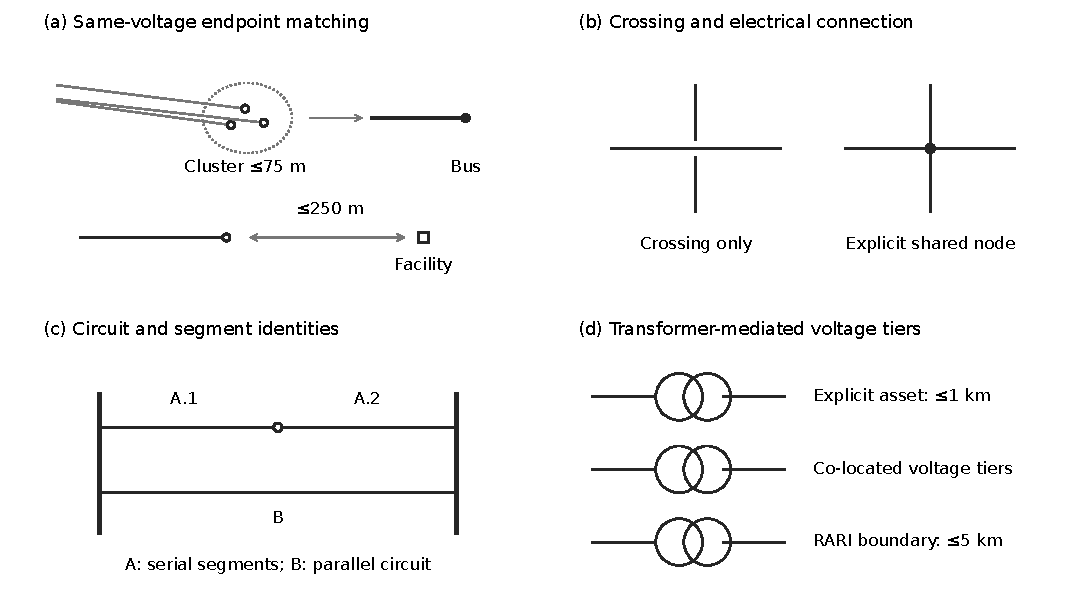
\includegraphics[keepaspectratio]{figures_final/fig01_network_reconstruction.pdf}}

\textbf{Figure 1---Connection rules used in static-network
reconstruction.} (a) Same-voltage endpoint clustering and facility
matching; (b) distinction between geometric crossings and explicit
shared nodes; (c) preservation of series segments and parallel-circuit
identity; and (d) cross-voltage connection from explicit equipment,
colocated facilities, and RARI boundary evidence. The diagrams are
abstract electrical schematics rather than geographic device locations.
Distance thresholds and fallback rules are listed in Table 3.

\PTneedspace{396pt}

\textbf{Table 3---Topology rules and thresholds.}

\begin{longtable}[]{@{}
  >{\raggedright\arraybackslash}p{(\linewidth - 4\tabcolsep) * \real{0.3333}}
  >{\raggedright\arraybackslash}p{(\linewidth - 4\tabcolsep) * \real{0.3333}}
  >{\raggedright\arraybackslash}p{(\linewidth - 4\tabcolsep) * \real{0.3333}}@{}}
\toprule\noalign{}
\begin{minipage}[b]{\linewidth}\raggedright
Object / step
\end{minipage} & \begin{minipage}[b]{\linewidth}\raggedright
Rule or threshold
\end{minipage} & \begin{minipage}[b]{\linewidth}\raggedright
Constraint / unmatched handling
\end{minipage} \\
\midrule\noalign{}
\endhead
\bottomrule\noalign{}
\endlastfoot
Distance coordinates & EPSG:3763; metres & Longitude and latitude stored
in WGS 84 \\
Endpoint clustering & 75 m within the same voltage & Different voltages
are not merged \\
Facility assignment & Same-voltage facility within 250 m & Create a
derived connection bus if unmatched \\
Facility normalization & Duplicate or colocated same-name facilities;
mobile facilities within 250 m of permanent stations & Retain merge
records \\
OSM splitting & Way endpoints or explicit shared nodes & Geometric
crossings do not create connections \\
Circuit identity & \texttt{\small circuit} /
\texttt{\small line\_\allowbreak{}section}; parallel circuits retained &
N−1 removes series model segments by physical circuit \\
Explicit transformer & Match high- and low-voltage buses within 1 km &
Preserve voltage-level consistency \\
Colocated transformer & Adjacent voltage levels in one OSM station &
Derived connection with evidence level retained \\
RARI boundary & Name-to-facility match within 5 km & May fall back to a
60 kV endpoint within 1 km of the high-voltage station \\
PDIRD parameter path & Length-weighted shortest path; model/source
length 0.65--1.60 & Use voltage-class proxy when rejected \\
Blocking checks & Self-loop, non-positive length, endpoint or voltage
conflict & Record and block invalid branches \\
\end{longtable}

\textbf{Table note.} Rules are defined in Section 2.2 and
\texttt{\small model\_\allowbreak{}config.\allowbreak{}json}. All
distances are projected planar distances. They are reconstruction rules,
not operator accuracy guarantees. Default electrical parameters and
coverage rules are reported in Supplementary Table S2.

\subsubsection{2.2.3 Evidence Applicability and Historical
Availability}\label{evidence-applicability-and-historical-availability}

Static-source dates and operating-case dates are versioned separately.
Only assets with an explicit commissioning date are switched by time.
Ordinary lines, transformers, and interconnections retain the frozen
static state when contemporaneous status records are unavailable.
Project documents support only the stated equipment and fields and are
not used to infer historical switching states. Cross-section scaling of
conductor resistance and transfer to other conductor families remain
engineering assumptions. Document pages, equipment identifiers, and
field-level judgements are stored in
\texttt{\small citation\_\allowbreak{}evidence\_\allowbreak{}ledger.\allowbreak{}csv};
Table 4 summarizes temporal handling.

\PTneedspace{234pt}

\textbf{Table 4---Source versions, validity dates, and case treatment.}

\begin{longtable}[]{@{}
  >{\raggedright\arraybackslash}p{(\linewidth - 4\tabcolsep) * \real{0.3333}}
  >{\raggedright\arraybackslash}p{(\linewidth - 4\tabcolsep) * \real{0.3333}}
  >{\raggedright\arraybackslash}p{(\linewidth - 4\tabcolsep) * \real{0.3333}}@{}}
\toprule\noalign{}
\begin{minipage}[b]{\linewidth}\raggedright
Object
\end{minipage} & \begin{minipage}[b]{\linewidth}\raggedright
Date or status evidence
\end{minipage} & \begin{minipage}[b]{\linewidth}\raggedright
Case treatment and limitation
\end{minipage} \\
\midrule\noalign{}
\endhead
\bottomrule\noalign{}
\endlastfoot
Ordinary lines and transformers & Historical status absent for most
individual devices & Frozen static state; not a complete historical
replay \\
New Minho--Galicia interconnection & REE announcement dated 2026-07-02 &
Disabled in every study case \\
Other Portugal--Spain interconnections & Maintenance and switching
histories unavailable & Fixed boundary equivalent; historical maps used
only to check corridor names (\hyperref[ref-REE2012]{REE, 2012}) \\
Generation and storage & 366 dated and 824 undated assets & Known dates
gate availability; unknown dates are treated as available and flagged \\
PDIRT/PDIRD and project evidence & Planning inventories, seasonal
profiles, or project records & Parameter, weight, and connection
evidence; no inference of real-time commissioning \\
\end{longtable}

\textbf{Table note.} In N1-3787, the capacity and voltage pair of the
three Estoi parallel equivalents are supported by a planning inventory,
but simultaneous availability and identical parameters remain model
assumptions (\hyperref[ref-REN2015Estoi]{REN, 2015}).

\subsection{2.3 Asset Mapping and Time-Series
Alignment}\label{asset-mapping-and-time-series-alignment}

\subsubsection{2.3.1 Asset Mapping and
Calendar}\label{asset-mapping-and-calendar}

The generation and storage inventory combines OSM, DGEG, and project
evidence. Plant and generator representations within 3 km and with
consistent capacity are merged. DGEG wind records replace incomplete OSM
wind capacities, and non-duplicate DGEG photovoltaic records supplement
OSM. Mapping priority is public connection evidence, declared voltage,
and then constrained spatial proximity. An asset without declared
voltage and with capacity of at least 100 MW searches only buses at 150
kV and above; smaller assets search buses at 60 kV and above. The
maximum distance is 20 km. Assets beyond this distance remain in the
inventory but are not injected. Assets commissioned after a case date
are unavailable; missing dates are treated as available and explicitly
flagged.

The common calendar uses
\texttt{\small interval\_\allowbreak{}start\_\allowbreak{}utc} as its
logical key. REN timestamps denote interval starts, whereas E-REDES
timestamps denote interval ends, as formalized in Equation (3):

\[
t_{\mathrm{E\text{-}REDES}}=t_{\mathrm{REN}}+15\ \mathrm{min}. \tag{3}\label{eq:time-alignment}
\]

Calendar days follow Europe/Lisbon civil time, giving 92 and 100
intervals on the spring and autumn daylight-saving transitions. REN
intra-day sequence numbers distinguish the repeated hour. E-REDES has no
fold marker, so duplicate station timestamps are averaged and flagged as
ambiguous. Missing intervals are not interpolated.

\subsubsection{2.3.2 Load, Generation, and
Storage}\label{load-generation-and-storage}

E-REDES energy is mapped to buses by facility code and converted to
nodal load. Equation (4) defines the unobserved national residual:

\[
R_t=P^{\mathrm{REN}}_{\mathrm{consumption},t}-\sum_j P^{\mathrm{EREDES}}_{j,t}. \tag{4}\label{eq:national-residual}
\]

Equation (5) assigns the residual to mapped delivery points using the
PDIRT public reference profile from the same season and closest
national-load condition (\hyperref[ref-ERSEPDIRT2024]{REN, 2024}):

\[
w_{j,t}=\frac{P^{\mathrm{PDIRT}}_{j,r(t)}}{\sum_{k\in\mathcal{M}}P^{\mathrm{PDIRT}}_{k,r(t)}},\qquad
P^{\mathrm{res}}_{j,t}=w_{j,t}R_t. \tag{5}\label{eq:residual-allocation}
\]

The profile provides only spatial weights and does not change the
15-minute resolution. E-REDES load uses a 0.97 power factor where
reactive power is not observed; residual load retains the PDIRT \(Q/P\)
relationship. Pumping and battery charging are distributed by mapped
storage capacity, with any remainder assigned to an explicit national
proxy. Nodal electric load must sum to REN
\texttt{\small Consumption + Storage} within 0.11 MW.

REN generation by technology is distributed among mapped and
commissioned assets of the same technology under
\(0\le P_{g,t}\le P_g^{\mathrm{nameplate}}\). Hydro and natural gas use
deterministic capacity-priority allocation, while other technologies use
available-capacity shares. Generation beyond mapped capacity is injected
at a designated 400 kV proxy bus as
\texttt{\small UNMAPPED\_\allowbreak{}NATIONAL\_\allowbreak{}RESIDUAL\_\allowbreak{}PROXY};
it must not be interpreted as the location of an omitted plant.

REN imports and exports are aligned to the common calendar but withheld
from boundary-power enforcement. Before solution, the pipeline checks
timestamps, required series, mapping completeness, load and generation
conservation, and capacity limits. Table 5 summarizes the executable
mapping and conservation rules; Supplementary Table S3 lists the
associated audit fields.

\PTneedspace{423pt}

\textbf{Table 5---Asset mapping and time-series transformation rules.}

\begin{longtable}[]{@{}
  >{\raggedright\arraybackslash}p{(\linewidth - 4\tabcolsep) * \real{0.3333}}
  >{\raggedright\arraybackslash}p{(\linewidth - 4\tabcolsep) * \real{0.3333}}
  >{\raggedright\arraybackslash}p{(\linewidth - 4\tabcolsep) * \real{0.3333}}@{}}
\toprule\noalign{}
\begin{minipage}[b]{\linewidth}\raggedright
Process
\end{minipage} & \begin{minipage}[b]{\linewidth}\raggedright
Rule
\end{minipage} & \begin{minipage}[b]{\linewidth}\raggedright
Audit or conservative treatment
\end{minipage} \\
\midrule\noalign{}
\endhead
\bottomrule\noalign{}
\endlastfoot
Asset deduplication & Merge plant/generator records within 3 km and with
consistent capacity & Preserve hierarchical deduplication status \\
Bus mapping & Public connection, declared voltage, then constrained
nearest bus & Maximum 20 km; retain but do not inject out-of-range
assets \\
Asset without declared voltage & Capacity ≥100 MW searches ≥150 kV;
otherwise ≥60 kV & Spatial proximity is not treated as connection
truth \\
Commissioning status & Disable when commissioning date is later than the
case & Treat unknown dates as available and flag them \\
Time labels & REN start; E-REDES end shifted by −15 min & Common key is
UTC interval start \\
Daylight saving / missing data & Lisbon civil days contain 92, 96, or
100 intervals & Average and flag repeated E-REDES station labels; no
interpolation \\
Energy to power & \(P(\mathrm{MW})=E(\mathrm{kWh})/250\) &
Interval-average power over 15 min \\
Direct load and residual & E-REDES observations plus PDIRT-weighted REN
consumption residual & pf=0.97 when Q is missing; retain residual Q/P \\
Pumping and battery charging & Positive values are electric load;
distribute by mapped storage capacity & Total load returns to
Consumption + Storage \\
Generation allocation & Same technology, mapped, commissioned, and
nameplate-constrained & Hydro/gas use capacity priority; others use
capacity share \\
Unmapped generation residual & Explicit national proxy-bus injection &
Must not be interpreted as a physical omitted-plant location \\
Cross-border exchange & REN imports/exports used only after solution &
Initial model solution determines boundary injections \\
\end{longtable}

\textbf{Table note.} The physical fields are named
\texttt{\small timestamp\_\allowbreak{}utc} in the calendar and monthly
databases;
\texttt{\small interval\_\allowbreak{}start\_\allowbreak{}utc} describes
their temporal semantics.

\subsection{2.4 Time-Indexed Case Generation and Alternating-Current
Power
Flow}\label{time-indexed-case-generation-and-alternating-current-power-flow}

Each 15-minute interval defines the steady-state case in Equation (6):

\[
C_t=(G,\theta,X_t,S_t,U_t,B_t), \tag{6}\label{eq:case-definition}
\]

where the static network \(G\) and parameters \(\theta\) are shared,
while operating inputs \(X_t\), device status \(S_t\), controls \(U_t\),
and boundary equivalent \(B_t\) vary with time. The principal dataset
contains one case per interval; sensitivity and application experiments
in Sections 4 and 5 use separately selected representative times.

\subsubsection{2.4.1 Case Assembly and
Solution}\label{case-assembly-and-solution}

Each case updates load, generation, equipment availability, seasonal
ratings, and boundary equivalents. An initial boundary solution
determines model net exchange. One angular reference is then retained,
and the other boundary nodes receive fixed active-power equivalents
distributed by public voltage and circuit count. Contemporaneous REN
exchange is used only for post-solution comparison.

AC power flow uses the pandapower Newton--Raphson implementation with DC
initialization (\hyperref[ref-Thurner2018]{Thurner et al., 2018}). The
principal workflow enforces reactive-power limits, resolves once after
boundary reconstruction, and performs a bounded tap search. Table 6
lists seasonal ratings, PV/PQ rules, compensation, reactors, boundary
weights, and numerical settings. These common settings are computational
proxies rather than operator control policies.

\subsubsection{2.4.2 Monthly Execution}\label{monthly-execution}

Cases are processed in parallel by civil month. Workers read inputs and
solve cases independently, whereas the parent process writes summaries,
state arrays, and audit bundles in one transaction. Re-runs skip
complete cases and retry failed cases. A month is complete only when
expected cases, completed cases, state arrays, and audit bundles agree.

\PTneedspace{342pt}

\textbf{Table 6---Case and solver settings.}

\begin{longtable}[]{@{}
  >{\raggedright\arraybackslash}p{(\linewidth - 4\tabcolsep) * \real{0.3333}}
  >{\raggedright\arraybackslash}p{(\linewidth - 4\tabcolsep) * \real{0.3333}}
  >{\raggedright\arraybackslash}p{(\linewidth - 4\tabcolsep) * \real{0.3333}}@{}}
\toprule\noalign{}
\begin{minipage}[b]{\linewidth}\raggedright
Item
\end{minipage} & \begin{minipage}[b]{\linewidth}\raggedright
Value or rule
\end{minipage} & \begin{minipage}[b]{\linewidth}\raggedright
Status
\end{minipage} \\
\midrule\noalign{}
\endhead
\bottomrule\noalign{}
\endlastfoot
Seasonal line rating & May--Sep ×1.00; Mar--Apr and Oct--Nov ×1.10;
Dec--Feb ×1.15 & Engineering proxy relative to summer base \\
PV threshold & Non-battery; installed capacity ≥20 MW and voltage ≥60 kV
& Remaining generation is PQ \\
PV voltage / reactive power & 1.0 p.u.; ±0.50 × installed MW in Mvar &
Uniform proxy \\
Load compensation & Target pf=0.98; maximum 15 Mvar per bus &
Engineering proxy \\
Shunt reactors & 5 × 150 Mvar at 400 kV & Explicitly flagged proxy
equipment \\
Boundary & One angle reference; other nodes weighted by voltage ×
circuit count & Not calibrated to measured REN exchange \\
AC algorithm & Newton--Raphson; DC initialization; enforce Q limits &
Maximum 50 iterations; tolerance \(10^{-6}\) MVA \\
Transformer taps & High-voltage side ±8 steps; 1.25\% per step; maximum
16 rounds & Target 0.985--1.015 p.u. \\
General screening & Voltage 0.90--1.10 p.u.; loading 100\% & Violations
retained; N−1 criteria defined separately \\
\end{longtable}

\textbf{Table note.} Settings come from the frozen
\texttt{\small model\_\allowbreak{}config.\allowbreak{}json} and monthly
execution code.

\subsection{2.5 Layered Storage, Provenance, and Quality
Control}\label{layered-storage-provenance-and-quality-control}

\subsubsection{2.5.1 Database and
Provenance}\label{database-and-provenance}

The main DuckDB stores sources in
\texttt{\small raw\_\allowbreak{}eredes},
\texttt{\small raw\_\allowbreak{}dgeg},
\texttt{\small raw\_\allowbreak{}osm},
\texttt{\small raw\_\allowbreak{}reference},
\texttt{\small raw\_\allowbreak{}documents}, and
\texttt{\small raw\_\allowbreak{}eredes\_\allowbreak{}aux}. The
\texttt{\small grid} and \texttt{\small geo} schemas store the static
network and geometry, \texttt{\small scenario} stores asset operating
points, \texttt{\small main} stores the common calendar and operating
series, and \texttt{\small provenance} stores file- and entity-level
lineage.

Each month has a separate result database.
\texttt{\small monthly\_\allowbreak{}model.\allowbreak{}cases} stores
one row per timestamp with status, summary metrics, and complete result
JSON. \texttt{\small bus\_\allowbreak{}order},
\texttt{\small line\_\allowbreak{}order}, and
\texttt{\small state\_\allowbreak{}arrays} store bus voltage and
line-loading arrays in fixed equipment order.
\texttt{\small audit\_\allowbreak{}bundles} preserve load, generation,
boundary, hotspot, and loss records. Views expand arrays to
equipment-long tables. The static model is copied once per monthly
database rather than repeated for every case.

Source records include URL, archive path, file size, and SHA-256.
\texttt{\small table\_\allowbreak{}lineage},
\texttt{\small raw\_\allowbreak{}record\_\allowbreak{}locator}, and
\texttt{\small entity\_\allowbreak{}evidence} provide table-, record-,
and evidence-level traceability. Each monthly
\texttt{\small run\_\allowbreak{}manifest} records input fingerprints
and case counts. Supplementary Table S5 provides the complete
data-layer, grain, and join-key inventory.

\subsubsection{2.5.2 Quality Control and
Recovery}\label{quality-control-and-recovery}

Quality control has four levels. Static checks cover keys, endpoints,
voltage, length, connectivity, and the boundary inventory. Time-series
checks cover temporal alignment, source completeness, load and
generation conservation, and capacity limits. Solver checks cover
convergence, voltage, loading, and the active-power-balance residual in
Equation (7):

\[
\varepsilon_t=P_t^{\mathrm{gen}}+P_t^{\mathrm{model,net}}-P_t^{\mathrm{load}}-P_t^{\mathrm{loss}}. \tag{7}\label{eq:power-balance}
\]

External checks use E-REDES national, municipal, substation, production,
and injection statistics that were excluded from nodal construction,
together with REN exchange and monthly loss reports. The 0.90--1.10 p.u.
voltage band and 100\% loading threshold are screening criteria;
violating cases remain in the release.

A case summary, state arrays, and audit bundle are committed in one
transaction. Any failure rolls back the full case and retains an error
record. Before formal monthly release, source and copy counts for
completed cases, arrays, and audit bundles must match. Supplementary
Table S4 lists thresholds, failure behavior, and record locations.

\section{3. Overview of the SimPT60
Dataset}\label{overview-of-the-simpt60-dataset}

SimPT60 comprises one main database and 11 monthly power-flow result
databases. The main database contains the static network, common time
series, source records, and validation observations. Monthly databases
contain the 15-minute cases and their solved states. The current static
model version is \texttt{\small PT60-v2.\allowbreak{}0.\allowbreak{}0}.

\subsection{3.1 Static Network Data}\label{static-network-data}

The static network contains 675 facilities, 3,783 buses, 4,943 lines,
228 transformers, 1,190 generation or storage units, 468 load points,
and seven Portugal--Spain boundary endpoints.
\texttt{\small grid.\allowbreak{}buses},
\texttt{\small grid.\allowbreak{}lines}, and
\texttt{\small grid.\allowbreak{}transformers} provide connectivity and
electrical parameters; \texttt{\small grid.\allowbreak{}generators},
\texttt{\small grid.\allowbreak{}load\_\allowbreak{}points}, and
\texttt{\small grid.\allowbreak{}interconnectors} link assets to buses.
Line and facility geometry is stored separately in
\texttt{\small geo.\allowbreak{}line\_\allowbreak{}geometries} and
\texttt{\small geo.\allowbreak{}facility\_\allowbreak{}geometries} to
avoid duplicating spatial objects in electrical tables.

Equipment tables retain \texttt{\small source},
\texttt{\small source\_\allowbreak{}status},
\texttt{\small parameter\_\allowbreak{}status}, and mapping-rule fields.
Users can build the complete pandapower network, select only devices
above an evidence threshold, or identify components whose parameters
were derived from public records or engineering proxies.

\PTneedspace{594.3pt}

Figure 2 shows the geographic network and one archived operating state.
Projection and cartography use GeoPandas
(\hyperref[ref-GeoPandas2026]{Fleischmann et al., 2026}).

\pandocbounded{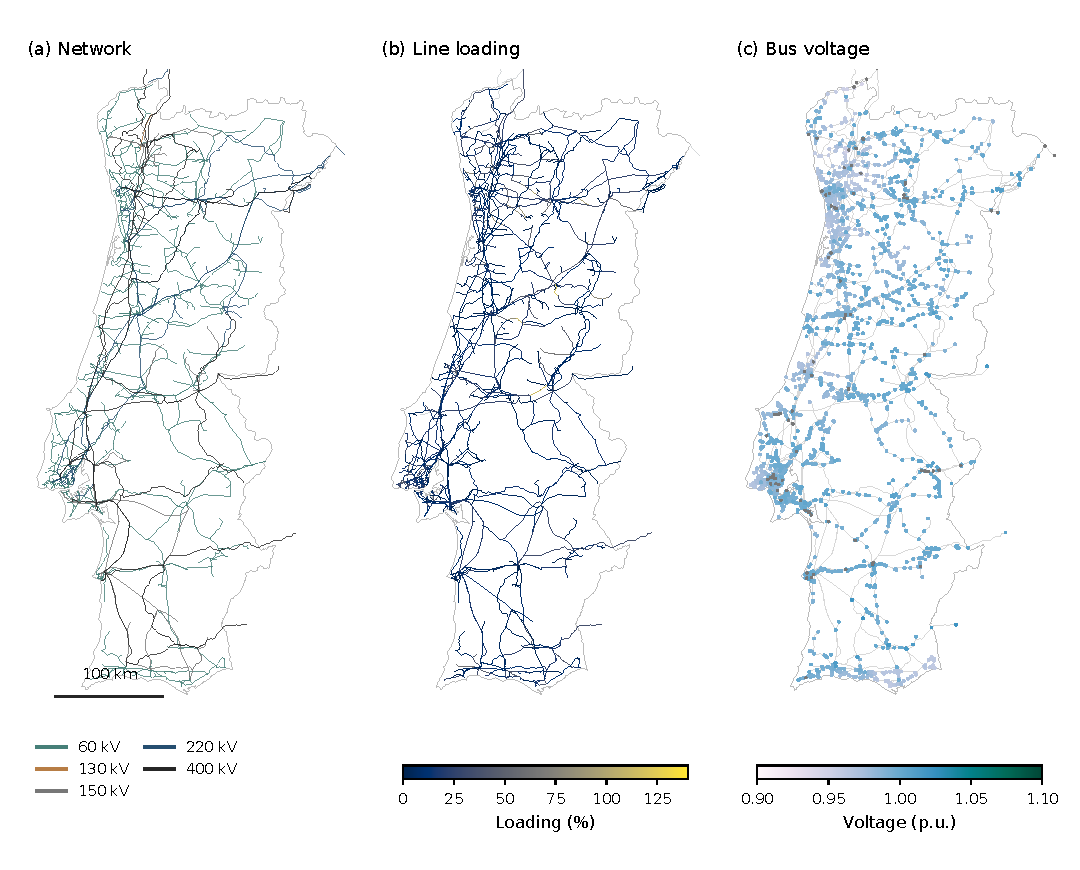
\includegraphics[keepaspectratio]{figures_final/fig02_geographic_network_state.pdf}}

\textbf{Figure 2---Geographic network and solved state at the annual
peak.} (a) The 60--400 kV network containing 3,783 buses and 4,943
lines; (b) line loading; and (c) bus voltage. All panels use EPSG:3763
with the same scale and extent, retain original line geometry and
Portugal--Spain boundary endpoints, and show a 100 km scale bar. The
operating state is the archived annual-peak model at 2026-01-15 12:15
UTC (load 11,329.2 MW), joined by stable equipment identifiers. Missing
solved states remain grey and are not imputed. The loading scale retains
values above 100\%. Values are modelled power flows, not telemetry.

\subsection{3.2 Time-Series Data}\label{time-series-data}

\texttt{\small main.\allowbreak{}interval\_\allowbreak{}calendar} is the
common index for all time series. It covers 328 civil days from
2025-05-01 to 2026-03-24 and contains 31,492 local 15-minute intervals.
Interval counts follow Europe/Lisbon daylight-saving transitions and
therefore need not equal the number of days multiplied by 96.

\texttt{\small main.\allowbreak{}eredes\_\allowbreak{}load} contains
12,360,502 load records for 397 substations. Raw records extend to
2026-03-25, but the joint modelling window ends on 2026-03-24.
\texttt{\small main.\allowbreak{}ren\_\allowbreak{}dispatch} contains
472,380 records across 15 national operating series for load, generation
by technology, storage, and cross-border exchange.
\texttt{\small main.\allowbreak{}weather\_\allowbreak{}hourly} holds
23,616 hourly records for Lisbon, Porto, and Faro;
\texttt{\small main.\allowbreak{}ren\_\allowbreak{}rnt\_\allowbreak{}balance}
contains 660 monthly balance records over 11 reporting periods.

The database also archives 14 E-REDES auxiliary datasets with 2,239,064
records. They cover national and municipal consumption, contracted
power, production, distribution-grid injection, distributed
self-consumption, seasonal substation loading, power quality, and
continuity of supply. These tables are excluded from nodal-power
construction and serve as withheld public observations in Section 4.

\subsection{3.3 Time-Indexed Power-Flow
Cases}\label{time-indexed-power-flow-cases}

Interval results are partitioned by civil month to limit file size and
support selective download. Eleven compact monthly databases map
one-to-one to the common calendar and contain 31,492 cases. Every case
in the present release completed AC power flow and is marked as
converged. October 2025 contains 2,980 intervals because daylight saving
time ends, whereas March 2026 covers only the first 24 days and contains
2,304 intervals.

Each case retains summary values, equipment-state arrays, and an
allocation audit bundle. Fixed \texttt{\small bus\_\allowbreak{}order}
and \texttt{\small line\_\allowbreak{}order} tables expand state arrays
to equipment-long form; the static device order is stored once per
month. Supplementary Table S5 lists fields and joins.

The main database also contains the N−1 application results from Section
5.
\texttt{\small scenario.\allowbreak{}annual\_\allowbreak{}nminus1\_\allowbreak{}snapshots}
records six representative times,
\texttt{\small scenario.\allowbreak{}annual\_\allowbreak{}nminus1\_\allowbreak{}results}
stores 9,894 contingency-level results, and
\texttt{\small scenario.\allowbreak{}annual\_\allowbreak{}nminus1\_\allowbreak{}overloads}
stores post-contingency overloaded circuits.
\texttt{\small scenario.\allowbreak{}nminus1\_\allowbreak{}control\_\allowbreak{}policy}
and
\texttt{\small provenance.\allowbreak{}annual\_\allowbreak{}nminus1\_\allowbreak{}runs}
record control-search bounds and experiment provenance. These
application tables remain separate from the continuous 15-minute cases
so that sampled security screening is not mistaken for continuous
operating observation.

\subsection{3.4 Dataset Coverage and
Composition}\label{dataset-coverage-and-composition}

\PTneedspace{540.7pt}

Figure 3 shows interval availability, the peak-load week, and monthly
case completeness.

\pandocbounded{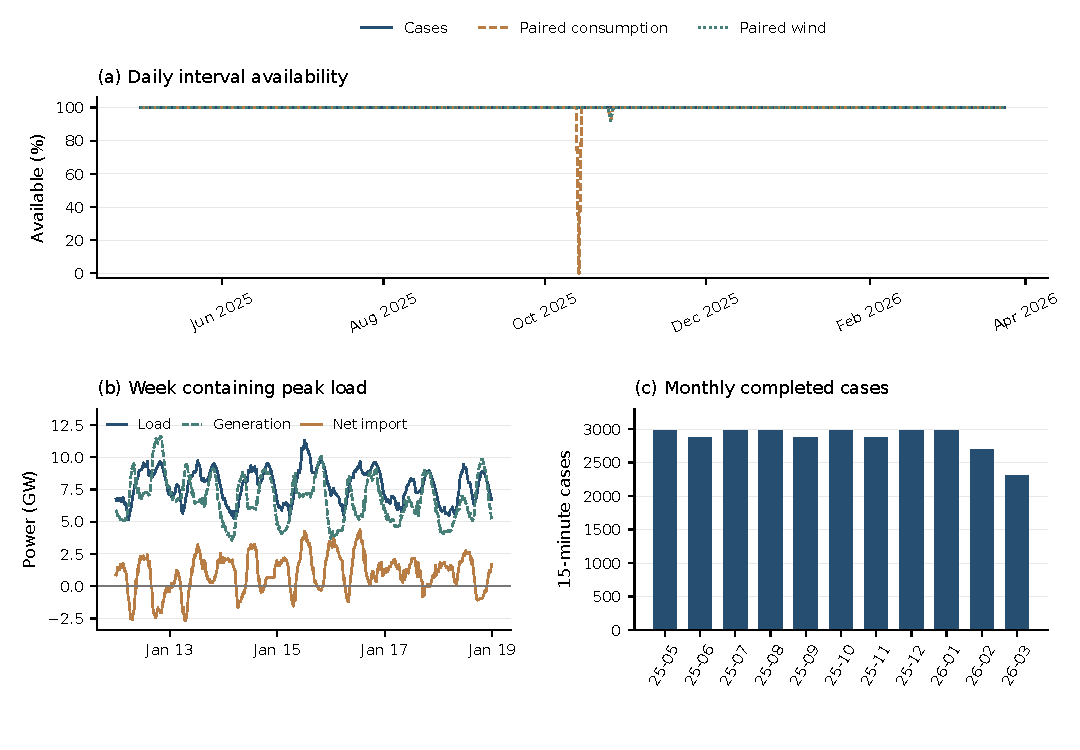
\includegraphics[keepaspectratio]{figures_final/fig03_temporal_coverage.pdf}}

\textbf{Figure 3---Temporal coverage and case completeness.} (a) Daily
fractions of available model cases, paired national-consumption
observations, and paired wind observations. Denominators follow Lisbon
civil days and daylight saving time; missing data are shown without
interpolation. (b) The complete civil week containing maximum system
load, with total electric load, generation, and REN net import. (c)
Completed and converged 15-minute cases by month, totaling 31,492. The
common window is 2025-05-01 to 2026-03-24; October contains the repeated
daylight-saving hour, and March is partial through day 24.

Table 7 summarizes the principal static, time-series, validation, and
application objects.

\PTneedspace{531pt}

\textbf{Table 7---Principal dataset statistics.}

\begin{longtable}[]{@{}
  >{\raggedright\arraybackslash}p{(\linewidth - 6\tabcolsep) * \real{0.2308}}
  >{\raggedright\arraybackslash}p{(\linewidth - 6\tabcolsep) * \real{0.2308}}
  >{\raggedleft\arraybackslash}p{(\linewidth - 6\tabcolsep) * \real{0.3077}}
  >{\raggedright\arraybackslash}p{(\linewidth - 6\tabcolsep) * \real{0.2308}}@{}}
\toprule\noalign{}
\begin{minipage}[b]{\linewidth}\raggedright
Category
\end{minipage} & \begin{minipage}[b]{\linewidth}\raggedright
Object
\end{minipage} & \begin{minipage}[b]{\linewidth}\raggedleft
Count
\end{minipage} & \begin{minipage}[b]{\linewidth}\raggedright
Basis
\end{minipage} \\
\midrule\noalign{}
\endhead
\bottomrule\noalign{}
\endlastfoot
Static & Facilities & 675 & Archived model inventory \\
Static & Buses & 3,783 & 2026-09-16 topology-validation snapshot \\
Static & Lines & 4,943 & Voltage-level coverage table \\
Static & Transformers & 228 & Topology-validation snapshot \\
Static & Generation / storage units & 1,190 & Asset inventory \\
Static & Load points & 468 & Load inventory \\
Static & Portugal--Spain boundary endpoints & 7 & Interconnection
inventory \\
Active network & Buses / lines & 3,664 / 4,787 & Connectivity
statistics \\
Time series & Common dates / intervals & 328 days / 31,492 & Common
calendar \\
Time series & Substation energy & 397 stations / 12,360,502 records &
Raw records through 2026-03-25 \\
Time series & REN national series & 15 types / 472,380 records & 15
min \\
Context & Weather & 3 locations / 23,616 records & Hourly \\
Context & REN monthly balance & 11 periods / 660 records & Monthly \\
Validation & E-REDES auxiliary products & 14 types / 2,239,064 records &
Multiple temporal resolutions \\
Power flow & Compact monthly databases / cases & 11 / 31,492 & Completed
and converged \\
Application & Full-element N−1 & 6 times / 9,894 cases & 1,649 elements
per time \\
\end{longtable}

\textbf{Table note.} Counts describe the released CORE-3783 variant. N−1
uses N1-3787. Section 3.6 and Supplementary Note S2 define their
object-level differences, section applicability, and fixed hashes.

\subsection{3.5 File Organization and
Distribution}\label{file-organization-and-distribution}

The frozen release comprises the analysis-ready main database, 11
monthly result databases, source and provenance records, and validation
and application results. Stable model identifiers join the static
network to the common calendar in the main database. Case identifiers
and fixed equipment order join summaries, state arrays, and audit
bundles in the monthly databases. Raw files are distributed when
licensing permits; otherwise, the release provides source metadata and
download scripts. \texttt{\small release.\allowbreak{}json},
\texttt{\small SHA256SUMS}, and the release README define file hashes,
the environment, and reproduction entry points.

\subsection{3.6 Frozen Release and Model-Version
Reconciliation}\label{frozen-release-and-model-version-reconciliation}

The paper freezes release \textbf{SimPT60-2026.09.21-r1}. The 31,492
historical cases and validation in Sections 3--4 use CORE-3783: 3,783
buses, 4,943 lines, and 228 transformers. The Section 5.2 N−1
demonstration uses N1-3787. In that variant, four colocated connection
nodes correct the Lanheses--Feitosa topology, and one merged Estoi
transformer object is separated into three parallel equivalent units.
The transformer table therefore contains 230 rows, although the three
Estoi units form one symmetric contingency group. Results from the two
variants cannot be interchanged and attributed to one model.
Supplementary Note S2 lists the required differences; the release
manifest records field-level differences and hashes.

\section{4. Validation}\label{validation}

No contemporaneous operator network model or branch-level state estimate
was available at the spatial extent of SimPT60. Validation therefore
does not target equipment-level error. It evaluates research
plausibility and usability through network structure, computational
consistency, sensitivity to modelling assumptions, and comparison with
public observations.

\subsection{4.1 Validation Design and Evidence
Levels}\label{validation-design-and-evidence-levels}

Validation has three layers. Public structural records and sensitivity
tests evaluate the network representation. E-REDES products withheld
from nodal-power construction evaluate aggregate temporal and spatial
behavior. Case completeness, convergence, and power balance evaluate
internal computational consistency. Comparisons are paired by common
timestamp or region without interpolation or removal of anomalous
months. Ninety-five-percent confidence intervals use clustered
resampling by civil day or spatial entity.

The evidence layers answer different questions. REN and E-REDES demand
and generation products do not share identical accounting boundaries,
and municipal or substation statistics are not line-flow truth. The
target is therefore research-level plausibility and usability rather
than equipment-level accuracy.

\subsection{4.2 Structural and Computational
Consistency}\label{structural-and-computational-consistency}

The full static network contains 3,783 buses, 4,943 lines, and 228
transformers. A single connected component contains 3,664 active buses
and 4,787 active lines. The simple-graph cycle rank is 501; median and
95th-percentile node degrees are 2 and 4. Model-to-public-background
route-km ratios at 60, 130, 150, 220, and 400 kV are 0.992, 1.090,
0.817, 0.819, and 1.033. REN aggregates provide the 150/220/400 kV
backgrounds. The 60/130 kV comparisons use non-independent OSM context
and cannot be interpreted as accuracy. The 130 kV ratio is based on only
seven model lines and is descriptive only.

Line parameters are a principal uncertainty. Of 4,240 60 kV lines, 1,517
have partial support from PDIRD circuit paths and 2,723 use
voltage-class engineering proxies. At 130--400 kV, every line is
classified as proxy at the line-level
\texttt{\small parameter\_\allowbreak{}status}. This overall
classification differs from field-level support, which Figure 4 reports
separately.

The 11 compact monthly databases contain 31,492 completed and converged
15-minute cases. The mean absolute AC closure residual across
generation, boundary exchange, load, and loss is \(1.77\times10^{-6}\)
MW, showing numerical agreement among released states and audit
quantities.

\PTneedspace{462.3pt}

\pandocbounded{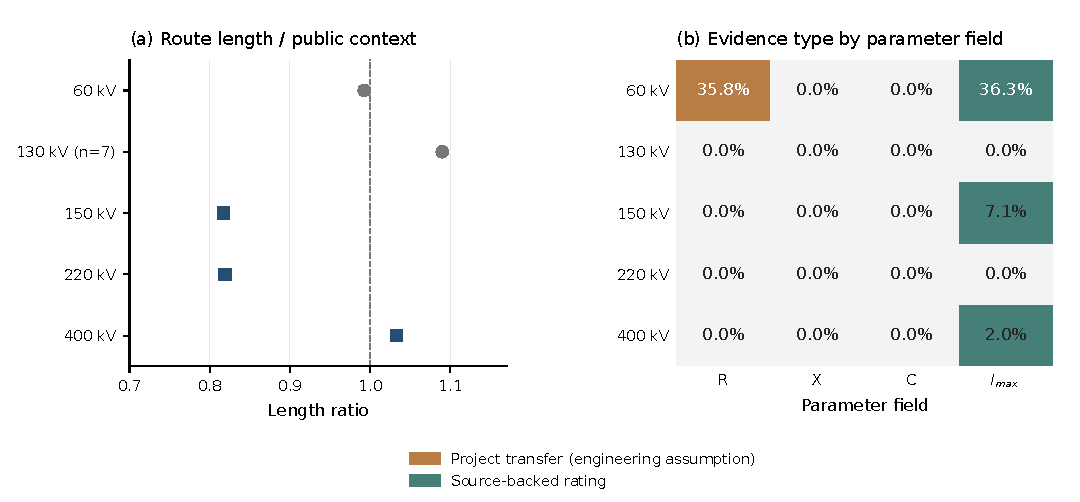
\includegraphics[keepaspectratio]{figures_final/fig04_network_parameter_evidence.pdf}}

\textbf{Figure 4---Structural coverage and field-level parameter
evidence.} (a) Model route-km divided by public background length for
each voltage class; the dashed line marks unity. Grey circles use
non-independent OSM context and blue squares use REN background.
Route-km and circuit length have different definitions, so the ratio is
not an accuracy measure. (b) Field-level separation of project-based
resistance transfer (orange; engineering assumption) and source-backed
ratings (green); cells show proportions. Grey denotes wholly proxy
fields. The 35.8\% resistance support is not direct observation and must
not be assigned the same evidence level as ratings. Reactance and
capacitance are proxies throughout. The 130 kV result contains seven
lines and is descriptive only. Table 8 reports line-level evidence
counts.

\PTneedspace{234pt}

\textbf{Table 8---Network structure, parameter evidence, and
computational completeness.}

\begin{longtable}[]{@{}
  >{\raggedleft\arraybackslash}p{(\linewidth - 12\tabcolsep) * \real{0.1481}}
  >{\raggedleft\arraybackslash}p{(\linewidth - 12\tabcolsep) * \real{0.1481}}
  >{\raggedleft\arraybackslash}p{(\linewidth - 12\tabcolsep) * \real{0.1481}}
  >{\raggedleft\arraybackslash}p{(\linewidth - 12\tabcolsep) * \real{0.1481}}
  >{\raggedleft\arraybackslash}p{(\linewidth - 12\tabcolsep) * \real{0.1481}}
  >{\raggedleft\arraybackslash}p{(\linewidth - 12\tabcolsep) * \real{0.1481}}
  >{\raggedright\arraybackslash}p{(\linewidth - 12\tabcolsep) * \real{0.1111}}@{}}
\toprule\noalign{}
\begin{minipage}[b]{\linewidth}\raggedleft
kV
\end{minipage} & \begin{minipage}[b]{\linewidth}\raggedleft
Buses
\end{minipage} & \begin{minipage}[b]{\linewidth}\raggedleft
Lines
\end{minipage} & \begin{minipage}[b]{\linewidth}\raggedleft
Route-km
\end{minipage} & \begin{minipage}[b]{\linewidth}\raggedleft
Background km
\end{minipage} & \begin{minipage}[b]{\linewidth}\raggedleft
Ratio
\end{minipage} & \begin{minipage}[b]{\linewidth}\raggedright
Line-level parameter evidence
\end{minipage} \\
\midrule\noalign{}
\endhead
\bottomrule\noalign{}
\endlastfoot
60 & 3,236 & 4,240 & 9,668.4 & 9,742.0 & 0.992 & 1,517 partial / 2,723
proxy \\
130 & 8 & 7 & 41.6 & 38.2 & 1.090 & 7 proxy \\
150 & 132 & 156 & 2,054.1 & 2,514.0 & 0.817 & 156 proxy \\
220 & 214 & 294 & 3,206.9 & 3,916.0 & 0.819 & 294 proxy \\
400 & 193 & 246 & 3,579.5 & 3,465.0 & 1.033 & 246 proxy \\
\end{longtable}

\textbf{Table note.} The 130 kV sample contains seven lines. Background
length is non-independent OSM context at 60/130 kV and REN aggregate
length at 150/220/400 kV. Route-km and circuit length differ, so ratios
are not accuracy. The active network is one connected component with
simple-graph cycle rank 501, median degree 2, and 95th-percentile degree
4. All 31,492 cases completed and converged; interval-weighted AC
closure MAE is \(1.77\times10^{-6}\) MW. Partial line-level support does
not mean that every field is observed; all \(x\) and \(c\) values are
proxies.

\subsection{4.3 Parameter and Spatial-Allocation
Sensitivity}\label{parameter-and-spatial-allocation-sensitivity}

Sensitivity experiments perturb line \(R/X\), capacitance, current
ratings, transformer capacity and impedance, and the spatial allocation
of load, generation, and boundary exchange at 22 representative times.
After shared baselines are removed, 264 cases remain and all converge.
The minimum Spearman correlation is 0.998 for line-impedance
perturbations and 0.993 for transformer perturbations. Current-rating
assumptions change maximum loading by as much as 34.48 percentage
points. System-wide rankings remain comparatively stable under spatial
alternatives, but allocating residual load by transformer capacity
reduces the Top-20 Jaccard index to 0.429. Specific hotspots are
consequently more assumption-dependent than the global ranking.

\PTneedspace{429.9pt}

Figure 5 summarizes ranking, hotspot-set, and maximum-loading responses.
Supplementary Table S6 contains all paired results. Hotspot persistence
shows that no line remains in the Top 20 across every annual time and
configuration (Supplementary Figure S1). Supplementary Table S7 reports
ablations of reactive-power limits, PV targets, compensation, reactors,
and tap control.

\pandocbounded{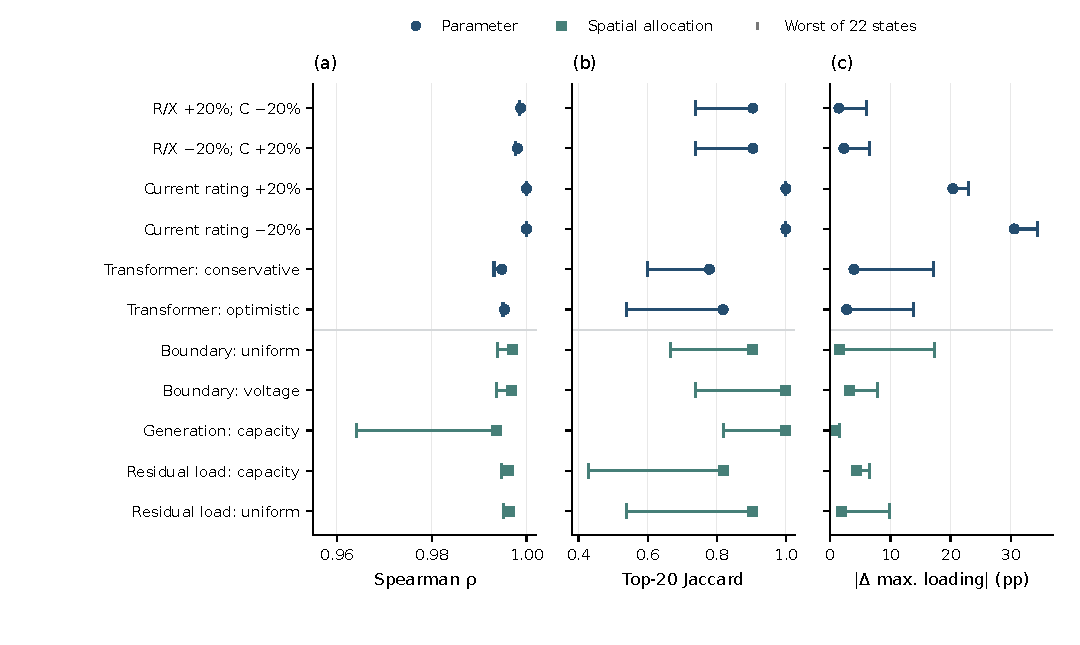
\includegraphics[keepaspectratio]{figures_final/fig05_parameter_spatial_sensitivity.pdf}}

\textbf{Figure 5---Sensitivity to parameters and spatial allocation.}
(a) Spearman correlation of line-loading ranks; (b) Top-20 Jaccard
index; and (c) absolute change in maximum loading. Markers denote
medians over 22 operating states and lines extend to the least favorable
result. The 154 parameter cases and 132 spatial cases share 22
baselines.

\subsection{4.4 External Temporal
Agreement}\label{external-temporal-agreement}

National demand comparison contains 31,388 paired intervals. The ratio
of mean SimPT60 consumption to public E-REDES consumption is 1.003, with
a day-block bootstrap 95\% confidence interval of {[}1.002, 1.005{]}.
Fifteen-minute Pearson correlation is 0.997 {[}0.996, 0.999{]}, and MAE
is 30.9 MW. Across 327 paired daily means, Pearson correlation is 0.995
and normalized RMSE is 0.013. October 2025 contains E-REDES missingness
and local deviations, but the month is retained
(\hyperref[ref-EREDESNationalConsumption]{E-REDES, n.d.-b}).

Wind comparison contains 31,484 paired intervals. The mean ratio between
SimPT60 and E-REDES distribution-grid wind injection is 1.056 {[}1.055,
1.058{]}, and Pearson correlation is 0.9998 {[}0.9997, 0.9998{]}.
Daily-mean correlation is also 0.9998. Photovoltaic correlation is
0.982, but mean national photovoltaic production in SimPT60 is
approximately 21.2 times distribution-grid injection. Hydro correlation
is 0.536. The latter comparisons span different accounting scopes and
are not absolute-scale validation
(\hyperref[ref-EREDESDistributionInjection]{E-REDES, n.d.-c};
\hyperref[ref-EREDESNationalProduction]{E-REDES, n.d.-d}).

\PTneedspace{680.0pt}

\pandocbounded{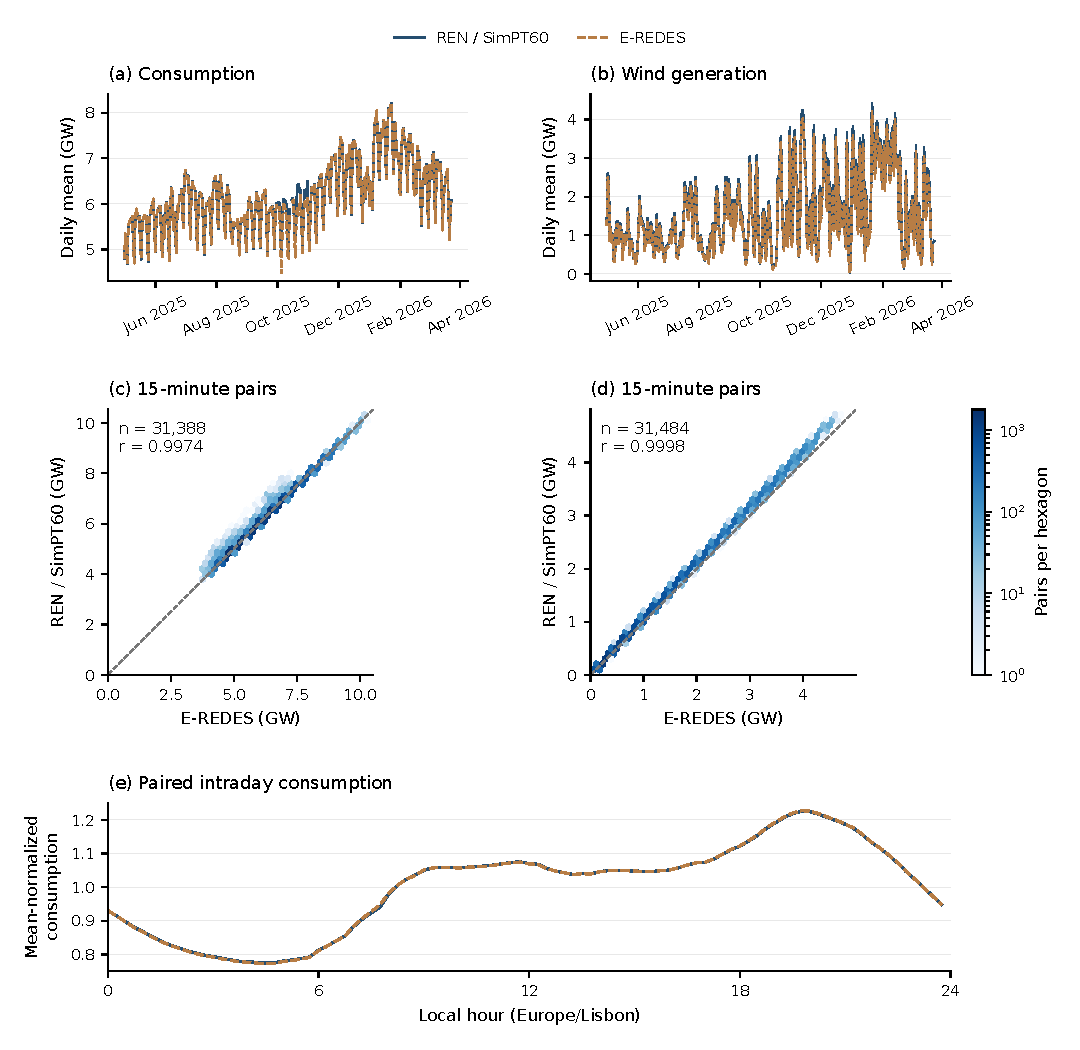
\includegraphics[keepaspectratio]{figures_final/fig07_temporal_validation.pdf}}

\textbf{Figure 6---External temporal validation of aggregate inputs.}
(a--b) Paired daily means for national consumption and wind; (c--d)
density of the corresponding 31,388 and 31,484 15-minute pairs, with a
shared logarithmic count scale, one-to-one line, and Pearson \(r\); and
(e) consumption profiles grouped by Lisbon local time and normalized by
each series' daily mean. Comparisons exclude only intervals missing a
required field and use no anomaly deletion, smoothing, or interpolation.
Consumption excludes pumping and battery charging and differs from total
electric load in the cases. Wind compares national production with
distribution-grid injection across different scopes. The figure
validates aggregate inputs, not nodal allocation or branch flow. Table 9
gives bootstrap intervals.

\subsection{4.5 External Spatial
Agreement}\label{external-spatial-agreement}

At municipal level, E-REDES monthly billed consumption is the reference
(\hyperref[ref-EREDESMunicipalityConsumption]{E-REDES, n.d.-e}). The
2,183 municipality-month pairs yield a Spearman correlation of 0.881,
with a 95\% confidence interval of {[}0.841, 0.910{]} from 199
municipality clusters; they cover 94.8\% of contemporaneous billed
energy. At substation level, 792 seasonal pairs yield a Spearman
correlation of 0.957 {[}0.946, 0.967{]} over 397 station clusters, a
mean ratio of 1.044, and MAE of 2.45 MW.

Municipality comparisons use the municipality containing each substation
as a proxy for its service area and therefore provide weak spatial
evidence. Seasonal substation loads come from the E-REDES capacity and
loading product (\hyperref[ref-EREDESSubstationCapacity]{E-REDES,
n.d.-a}). They test facility ranking and scale, but share the same
operator as the 15-minute load data and are not fully independent nodal
truth.

\PTneedspace{434.3pt}

\pandocbounded{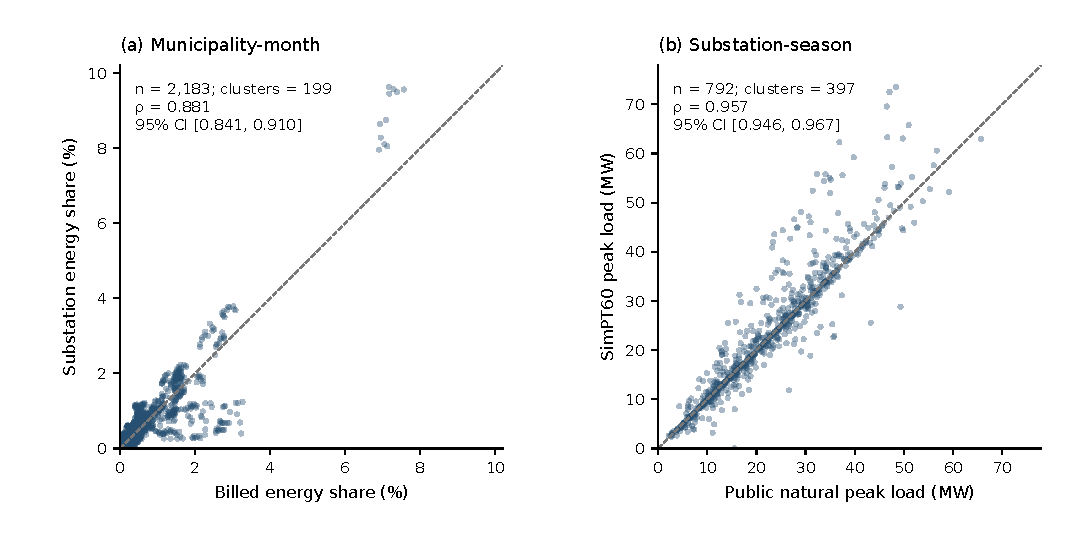
\includegraphics[keepaspectratio]{figures_final/fig08_spatial_validation.pdf}}

\textbf{Figure 7---Spatial agreement at municipality and substation
levels.} (a) 2,183 municipality-month load-share pairs; (b) 792 seasonal
substation-peak pairs. Axes have equal scale and dashed one-to-one
lines. Labels report Spearman correlation and archived 1,000-replicate
cluster-bootstrap 95\% intervals using 199 municipality and 397
substation clusters; bands are not regression intervals. Municipality
assignment is a weak service-area proxy, and cross-product evidence from
the same operator is not fully independent nodal truth.

\PTneedspace{261pt}

\textbf{Table 9---Summary of cross-source validation.}

\begin{longtable}[]{@{}
  >{\raggedright\arraybackslash}p{(\linewidth - 6\tabcolsep) * \real{0.2308}}
  >{\raggedleft\arraybackslash}p{(\linewidth - 6\tabcolsep) * \real{0.3077}}
  >{\raggedright\arraybackslash}p{(\linewidth - 6\tabcolsep) * \real{0.2308}}
  >{\raggedright\arraybackslash}p{(\linewidth - 6\tabcolsep) * \real{0.2308}}@{}}
\toprule\noalign{}
\begin{minipage}[b]{\linewidth}\raggedright
Validation target
\end{minipage} & \begin{minipage}[b]{\linewidth}\raggedleft
Samples or independent blocks
\end{minipage} & \begin{minipage}[b]{\linewidth}\raggedright
Result (95\% CI)
\end{minipage} & \begin{minipage}[b]{\linewidth}\raggedright
Evidence level
\end{minipage} \\
\midrule\noalign{}
\endhead
\bottomrule\noalign{}
\endlastfoot
National consumption & 31,388 intervals / 327 days & Mean ratio 1.003
{[}1.002, 1.005{]}; \(r=0.997\) {[}0.996, 0.999{]} & REN--E-REDES
consumption; reference includes losses \\
Wind & 31,484 intervals / 328 days & Mean ratio 1.056 {[}1.055,
1.058{]}; \(r=0.9998\) {[}0.9997, 0.9998{]} & REN--E-REDES
distribution-injection corroboration \\
Photovoltaic temporal variation & 31,484 intervals / 328 days &
\(r=0.982\) {[}0.979, 0.984{]}; absolute scale not comparable & National
production versus distribution injection \\
Municipal load share & 2,183 pairs / 199 municipalities & \(\rho=0.881\)
{[}0.841, 0.910{]} & Same operator across datasets; weak spatial
proxy \\
Seasonal substation peak & 792 pairs / 397 stations & \(\rho=0.957\)
{[}0.946, 0.967{]} & Same operator across datasets \\
AC power closure & 31,492 cases & MAE \(1.77\times10^{-6}\) MW &
Internal physical consistency \\
\end{longtable}

\subsubsection{4.5.1 Station-Held-Out Spatial Reconstruction
Test}\label{station-held-out-spatial-reconstruction-test}

A station-held-out experiment divides 394 matched stations into five
deterministic folds. At 22 times, it compares global capacity share,
five geographically nearest stations, and five nearest stations along
the reconstructed network, yielding 8,541 observation pairs. Table 10
shows that network-neighbor MAE is approximately 9.9\% below global
capacity share, but is not lower than geographic-neighbor MAE and has an
overlapping confidence interval. Reconstructed connectivity therefore
contains useful proximity information but does not independently recover
precise nodal demand. Supplementary Note S3 specifies folds, distance
weights, and bootstrap procedures.

\PTneedspace{180pt}

\textbf{Table 10---Station-held-out spatial-allocation results.}

\begin{longtable}[]{@{}
  >{\raggedright\arraybackslash}p{(\linewidth - 8\tabcolsep) * \real{0.1667}}
  >{\raggedleft\arraybackslash}p{(\linewidth - 8\tabcolsep) * \real{0.2222}}
  >{\raggedright\arraybackslash}p{(\linewidth - 8\tabcolsep) * \real{0.1667}}
  >{\raggedleft\arraybackslash}p{(\linewidth - 8\tabcolsep) * \real{0.2222}}
  >{\raggedleft\arraybackslash}p{(\linewidth - 8\tabcolsep) * \real{0.2222}}@{}}
\toprule\noalign{}
\begin{minipage}[b]{\linewidth}\raggedright
Method
\end{minipage} & \begin{minipage}[b]{\linewidth}\raggedleft
Stations / observation pairs
\end{minipage} & \begin{minipage}[b]{\linewidth}\raggedright
MAE (MW), 95\% CI
\end{minipage} & \begin{minipage}[b]{\linewidth}\raggedleft
RMSE (MW)
\end{minipage} & \begin{minipage}[b]{\linewidth}\raggedleft
WAPE
\end{minipage} \\
\midrule\noalign{}
\endhead
\bottomrule\noalign{}
\endlastfoot
Capacity share & 394 / 8,541 & 4.729 {[}4.412, 5.063{]} & 6.357 &
38.4\% \\
Five geographic neighbors & 394 / 8,541 & 4.249 {[}3.972, 4.544{]} &
5.675 & 34.5\% \\
Five network-path neighbors & 394 / 8,541 & 4.262 {[}3.971, 4.545{]} &
5.702 & 34.6\% \\
\end{longtable}

\subsection{4.6 Generation Scope and Quantified Dependence on Spatial
Proxies}\label{generation-scope-and-quantified-dependence-on-spatial-proxies}

Directly observed load accounts for 67.93--74.93\% of monthly
consumption; the remaining 25.07--32.07\% is allocated with PDIRT
reference profiles. National generation proxies account for only
0.010--0.063\% of monthly generation, but this national average hides
small technology classes. In May 2025, proxy shares reach 90.58\% for
batteries and 11.07\% for other thermal generation. Aggregate balance
therefore does not establish reliable local asset location.

\PTneedspace{680.0pt}

All non-rounding generation proxies are injected at one 400 kV receiving
bus, which represents a model balancing location only. Figure 8 shows
consumption residuals, technology-level generation proxies, and their
spatial distribution by latitude band. Monthly values for eight
technologies, interval flags, and bus-level details are released as CSV.

\pandocbounded{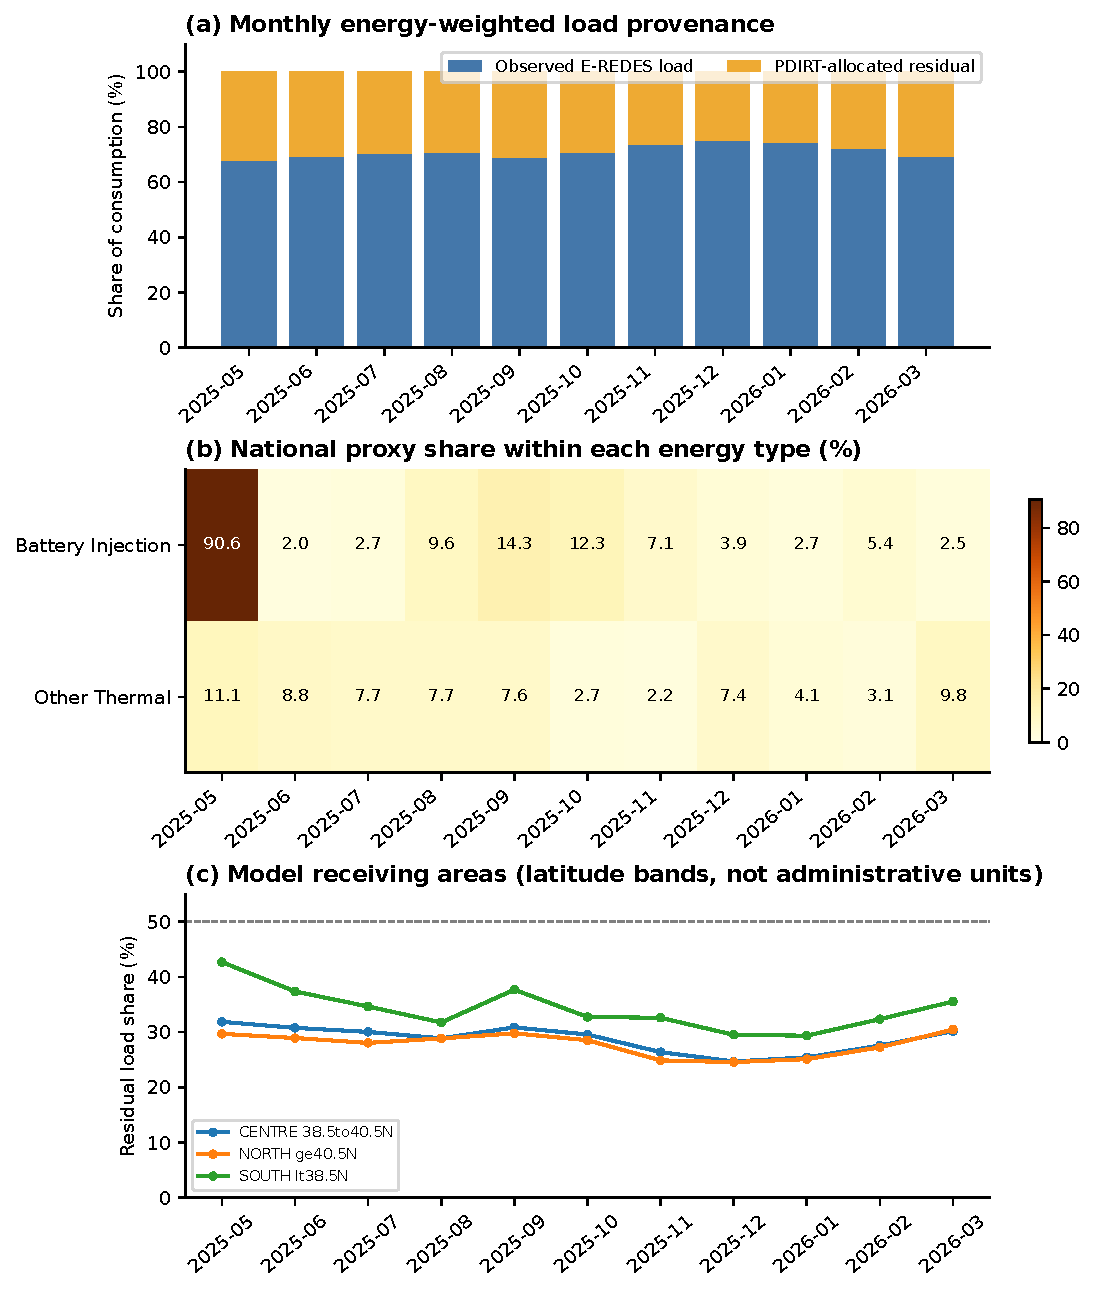
\includegraphics[keepaspectratio]{figures_final/fig10_proxy_provenance.pdf}}

\textbf{Figure 8---Temporal and spatial distribution of observed and
proxy power.} (a) Observed consumption and the PDIRT-allocated residual;
(b) technology-level proxy shares for batteries and other thermal
generation; and (c) load-residual share by latitude band of receiving
buses. Panels use different denominators. Regions denote allocation
locations in the model, not the true locations of missing assets.

\subsection{4.7 Limitations}\label{limitations}

Validation supports aggregate temporal agreement, plausible spatial
ranking, and numerical self-consistency. Parameter and allocation
perturbations also show that system-wide trends are generally stable.
Public information remains insufficient to validate device-by-device
topology, branch flows, switching status, or generator capability.
Correlation, convergence, and screening counts must therefore not be
interpreted as equipment-level accuracy of an operator network. SimPT60
is intended for reproducible research cases, relative-risk comparison,
and method testing. Real-time dispatch, protection settings, and formal
compliance assessment require contemporaneous operator-approved models
and operating records.

\section{5. Application}\label{application}

Two compact experiments demonstrate deterministic scenario comparison
and batch contingency computation. They illustrate model use and are
neither operational forecasts nor formal compliance assessments.

\subsection{5.1 Deterministic Grid-Stress
Scenario}\label{deterministic-grid-stress-scenario}

\PTneedspace{336.9pt}

Starting from 2026-01-20 19:45 UTC, nodal load, generation by
technology, and boundary exchange are scaled jointly from 0.90 to 1.15
and solved independently. All five scenarios converge. Maximum line
loading is 96.10\% at baseline, reaches 100.50\% with three overloaded
lines at 1.05, and reaches 109.41\% at 1.15. Minimum voltage remains
above 0.90 p.u. Figure 9 shows loading and voltage responses; exact
scenario results are released as CSV.

\pandocbounded{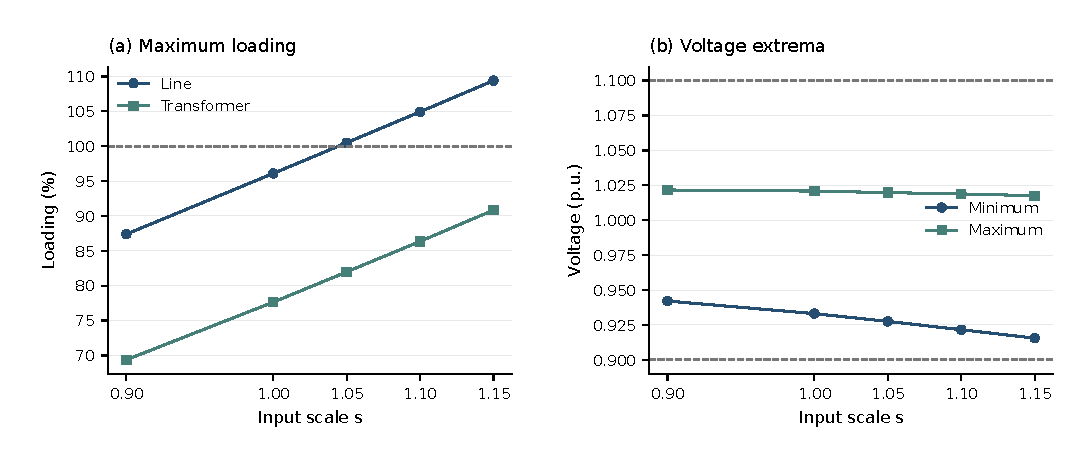
\includegraphics[keepaspectratio]{figures_final/fig11_grid_stress.pdf}}

\textbf{Figure 9---Deterministic grid-stress response.} (a) Maximum line
and transformer loading; (b) minimum and maximum bus voltage. Dashed
lines mark 100\% line loading and the 0.90--1.10 p.u. screening band.
Connecting lines guide the eye only.

\subsection{5.2 Representative-Time Full-Element N−1
Demonstration}\label{representative-time-full-element-n1-demonstration}

Six times are selected in advance from the continuous series: maximum
and minimum load, maximum wind, maximum photovoltaic generation, maximum
net import, and maximum net export. The same 1,649 contingencies are
used at each time in N1-3787: 1,421 line-circuit groups and 228
transformer groups. Series model segments are removed together, while
one unit is removed from a parallel equivalent. Supplementary Table S8
specifies selection and exclusion rules.

\PTneedspace{680.0pt}

The six times produce 9,894 cases, of which 9,888 converge under the
principal solution. Absolute screening passes 6,048 cases, and 9,064
cases have neither a new violation relative to N−0 nor a material
island. The latter is an auxiliary diagnostic; it does not identify
every worsening of a pre-existing violation and does not replace
absolute criteria. Figure 10 and Table 11 report the results; complete
membership and case-level outputs are preserved in the repository.

\pandocbounded{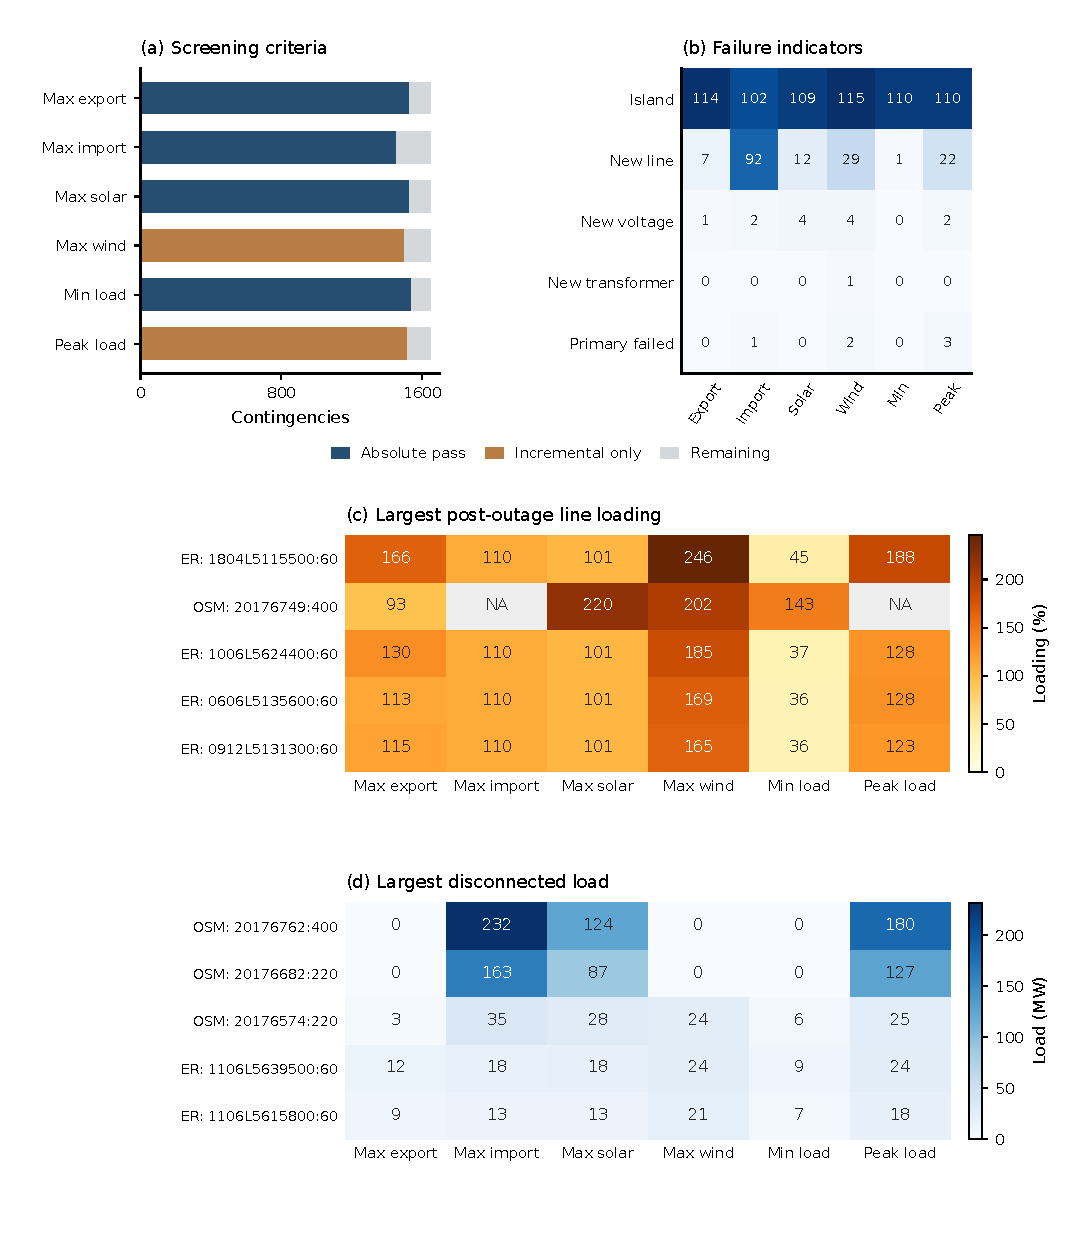
\includegraphics[keepaspectratio]{figures_final/fig12_annual_nminus1.pdf}}

\textbf{Figure 10---Full-element N−1 screening at representative times.}
(a) Absolute and incremental diagnostics; (b) material islands, new
violations, and principal-solution failures; (c--d) elements associated
with the highest post-contingency line loading and largest disconnected
load. Supplementary Note S4 defines the complete criteria and quantifies
worsening of pre-existing violations.

\PTneedspace{288pt}

\textbf{Table 11---Full-element N−1 results at six representative
times.}

\begin{longtable}[]{@{}
  >{\raggedright\arraybackslash}p{(\linewidth - 10\tabcolsep) * \real{0.1304}}
  >{\raggedleft\arraybackslash}p{(\linewidth - 10\tabcolsep) * \real{0.1739}}
  >{\raggedleft\arraybackslash}p{(\linewidth - 10\tabcolsep) * \real{0.1739}}
  >{\raggedleft\arraybackslash}p{(\linewidth - 10\tabcolsep) * \real{0.1739}}
  >{\raggedleft\arraybackslash}p{(\linewidth - 10\tabcolsep) * \real{0.1739}}
  >{\raggedleft\arraybackslash}p{(\linewidth - 10\tabcolsep) * \real{0.1739}}@{}}
\toprule\noalign{}
\begin{minipage}[b]{\linewidth}\raggedright
Snapshot
\end{minipage} & \begin{minipage}[b]{\linewidth}\raggedleft
Cases
\end{minipage} & \begin{minipage}[b]{\linewidth}\raggedleft
Principal solution converged
\end{minipage} & \begin{minipage}[b]{\linewidth}\raggedleft
Absolute screen passed
\end{minipage} & \begin{minipage}[b]{\linewidth}\raggedleft
No new violation and no material island
\end{minipage} & \begin{minipage}[b]{\linewidth}\raggedleft
Material island
\end{minipage} \\
\midrule\noalign{}
\endhead
\bottomrule\noalign{}
\endlastfoot
Maximum net export & 1,649 & 1,649 & 1,527 & 1,527 & 114 \\
Maximum net import & 1,649 & 1,648 & 1,455 & 1,455 & 102 \\
Maximum photovoltaic & 1,649 & 1,649 & 1,526 & 1,526 & 109 \\
Maximum wind & 1,649 & 1,647 & 0 & 1,502 & 115 \\
Minimum load & 1,649 & 1,649 & 1,538 & 1,538 & 110 \\
Maximum load & 1,649 & 1,646 & 2 & 1,516 & 110 \\
Total & 9,894 & 9,888 & 6,048 & 9,064 & 660 \\
\end{longtable}

\textbf{Table note.} Absolute pass, no-new-violation/no-material-island,
and material-island columns are computed separately and are not mutually
exclusive and exhaustive classes. At maximum net export, eight
additional non-islanding cases have new violations: seven line-thermal
and one voltage violation. Together with 1,527 no-new-violation cases
and 114 material islands, they account for all 1,649 cases.

These applications support relative scenarios and diagnostic contingency
screening. Equipment-level interpretation remains limited by the
parameter, status, and control evidence summarized in Section 4.7.

\section{6. Conclusions}\label{conclusions}

SimPT60 links a public-data reconstruction of the continental Portuguese
60--400 kV network to 31,492 consecutive 15-minute AC power-flow states
in one traceable, versioned product. CORE-3783 contains 3,783 buses,
4,943 lines, and 228 transformer objects, connected to source records,
allocation rules, and solution outputs by stable identifiers.

Validation supports aggregate spatiotemporal agreement and numerical
self-consistency. National load and wind correlations are approximately
0.997 and 0.9998. Spearman correlations for municipal and substation
spatial rankings are 0.881 and 0.957. The station-held-out experiment
shows that network proximity improves on global capacity allocation but
not on geographic proximity. System-wide rankings are generally stable
under parameter and allocation perturbations, whereas individual
hotspots and absolute loading remain sensitive to proxy assumptions.

The grid-stress scenarios and 9,894 N−1 cases at six representative
times demonstrate support for scenario analysis and batch contingency
computation. These results compare model states and identify elements
for further investigation; they do not constitute security
certification.

SimPT60 is a public-data-derived research dataset. It is not an operator
internal model, state estimate, or digital twin. Equipment-level
validation will require contemporaneous device status, generator P--Q
capability, switching configuration, and post-contingency actions.

\section{Data Availability}\label{data-availability}

The frozen \textbf{SimPT60-2026.09.21-r1} release is available from the
\href{https://github.com/MingLeiZhou/PortugueseOPD/releases/tag/SimPT60-2026.09.21-r1}{project's
versioned GitHub release}. It contains the reproducibility core, 11
compressed monthly result databases, the monthly manifest,
\texttt{\small release.\allowbreak{}json}, and
\texttt{\small SHA256SUMS}. Raw third-party files are redistributed only
when their licences permit; otherwise, the release retains source URLs,
archived metadata, file sizes, fingerprints, and retrieval instructions.
The release manifest identifies the CORE-3783 and N1-3787 model variants
and their permitted uses.

\section{Code Availability}\label{code-availability}

Reproduction code, the locked Python environment, and the minimal replay
commands are included in the same
\href{https://github.com/MingLeiZhou/PortugueseOPD/releases/tag/SimPT60-2026.09.21-r1}{SimPT60-2026.09.21-r1
release}. The immutable tag fixes the release state, while
\texttt{\small release.\allowbreak{}json} and
\texttt{\small CODE\_\allowbreak{}VERSION.\allowbreak{}json} record the
implementation commit and the limitation that the original historical
monthly runs did not store a code commit. The replay workflow verifies
selected released cases at a tolerance of \(10^{-5}\) in the units of
each compared field.

\section{References}\label{references}

\phantomsection\label{ref-APA3403}

APA (2021).
\href{https://siaia.apambiente.pt/AIADOC/AIA3403/parecerca_3403202192134944.pdf}{Sobreequipamento
do Parque Eólico de Trancoso: Parecer da Comissão de Avaliação, AIA
3403}. July; PDF p.~5.

\phantomsection\label{ref-APAPPA421}

APA (n.d.-a).
\href{https://siaia.apambiente.pt/PosAvaliacao/DetalhesPosAvaliacao/421}{PPA
421: Sub-Parque Eólico de Sernancelhe e ligação a Moimenta}. AIA 2009;
project-name and operation-date fields; archived 2026-09-21.

\phantomsection\label{ref-APAPPA407}

APA (n.d.-b).
\href{https://siaia.apambiente.pt/PosAvaliacao/DetalhesPosAvaliacao/407}{PPA
407: Ligação do Douro Sul à Subestação de Armamar e Subestação de
Moimenta}. AIA 2009; archived 2026-09-21.

\phantomsection\label{ref-DGEGPNEC2030Revision2024}

DGEG (2024).
\href{https://www.dgeg.gov.pt/media/54fldci3/pnec2030_para_aprov_ar.pdf}{Portugal:
Plano Nacional Energia e Clima 2021--2030, atualização/revisão}. DGEG.

\phantomsection\label{ref-DGEGGeo2026}

DGEG (n.d.).
\href{https://www.dgeg.gov.pt/pt/servicos-online/setor-energetico/}{Informação
Geográfica de Energia Elétrica}. Official geographic data portal.
Accessed 2026-09-21.

\phantomsection\label{ref-Tocha2019}

EDP Distribuição (2019).
\href{https://siaia.apambiente.pt/AIADOC/AIA3274/projeto\%20linha\%20eletrica\%20pe\%20tocha\%20ii2019729153214.pdf}{Memória
Descritiva e Justificativa: Linha a 60 kV PE Tocha II--Tocha}. 19
February; process 2800-19C007374; PDF pp.~3, 5.

\phantomsection\label{ref-EREDESPDIRD2020AnnexB}

E-REDES; Entidade Reguladora dos Serviços Energéticos (2020).
\href{https://www.erse.pt/media/340hrot0/proposta-pdird-e-2020_anexo_b.pdf}{PDIRD-E
2020, Anexo B}. ERSE. July version; northern circuit records: PDF
pp.~93--95.

\phantomsection\label{ref-EREDESSubstationCapacity}

E-REDES (n.d.-a).
\href{https://e-redes.opendatasoft.com/explore/dataset/carga-na-subestacao/}{Carga
na subestação}. E-REDES Open Data Portal. Accessed 2026-09-21.

\phantomsection\label{ref-EREDESNationalConsumption}

E-REDES (n.d.-b).
\href{https://e-redes.opendatasoft.com/explore/dataset/consumo-total-nacional/}{Consumo
total nacional}. E-REDES Open Data Portal. Accessed 2026-09-21.

\phantomsection\label{ref-EREDESDistributionInjection}

E-REDES (n.d.-c).
\href{https://e-redes.opendatasoft.com/explore/dataset/energia-injetada-na-rede-de-distribuicao/}{Energia
injetada na rede de distribuição}. E-REDES Open Data Portal. Accessed
2026-09-21.

\phantomsection\label{ref-EREDESNationalProduction}

E-REDES (n.d.-d).
\href{https://e-redes.opendatasoft.com/explore/dataset/energia-produzida-total-nacional/}{Energia
produzida total nacional}. E-REDES Open Data Portal. Accessed
2026-09-21.

\phantomsection\label{ref-EREDESMunicipalityConsumption}

E-REDES (n.d.-e).
\href{https://e-redes.opendatasoft.com/explore/dataset/3-consumos-faturados-por-municipio-ultimos-10-anos/}{Monthly
consumption by municipality}. E-REDES Open Data Portal. Accessed
2026-09-21.

\phantomsection\label{ref-EREDESRND2026}

E-REDES (n.d.-f).
\href{https://e-redes.opendatasoft.com/pages/rnd/}{Rede Nacional de
Distribuição: Dados da Rede AT e Cargas de Subestação}. Open data
portal. Accessed 2026-09-21.

\phantomsection\label{ref-GISCO2024}

Eurostat GISCO (2024).
\href{https://gisco-services.ec.europa.eu/distribution/v2/countries/}{Countries
2024: Portugal Boundary, 1:1 Million, EPSG:4326}. Geospatial dataset.
Accessed 2026-09-21.

\phantomsection\label{ref-GeoPandas2026}

Fleischmann, Martin; Van den Bossche, Joris; Jordahl, Kelsey; Richards,
Matthew John; McBride, James; Wasserman, Jacob; Ward, Brendan; Wolf,
Levi John (2026).
\href{https://doi.org/10.1016/j.compenvurbsys.2026.102495}{GeoPandas:
Fundamental Data Structures for Vector Spatial Data in Python}.
\emph{Computers, Environment and Urban Systems}, 130, 102495.
Author/year/DOI verified against the official GeoPandas CITATION.md and
Crossref on 2026-09-21; assigned issue December 2026, not asserted as
the online publication date.

\phantomsection\label{ref-GeofabrikPortugal2026}

Geofabrik GmbH (n.d.).
\href{https://download.geofabrik.de/europe/portugal.html}{OpenStreetMap
Data Extract for Portugal}. Geospatial data extract. Accessed
2026-09-21.

\phantomsection\label{ref-Horsch2018}

Hörsch, Jonas; Hofmann, Fabian; Schlachtberger, David; Brown, Tom
(2018). \href{https://doi.org/10.1016/j.esr.2018.08.012}{PyPSA-Eur: An
Open Optimisation Model of the European Transmission System}.
\emph{Energy Strategy Reviews}, 22, 207-215.

\phantomsection\label{ref-Meinecke2020}

Meinecke, Steffen; Sarajlić, Džanan; Drauz, Simon Ruben; Klettke,
Annika; Lauven, Lars-Peter; Rehtanz, Christian; Moser, Albert; Braun,
Martin (2020). \href{https://doi.org/10.3390/en13123290}{SimBench---A
Benchmark Dataset of Electric Power Systems to Compare Innovative
Solutions Based on Power Flow Analysis}. \emph{Energies}, 13(12), 3290.

\phantomsection\label{ref-OpenInfraMap2026}

OpenInfraMap contributors (n.d.).
\href{https://openinframap.org/about}{OpenInfraMap}. Web map of
infrastructure data derived from OpenStreetMap. Accessed 2026-09-21.

\phantomsection\label{ref-OSM2026}

OpenStreetMap contributors (n.d.).
\href{https://www.openstreetmap.org/copyright}{OpenStreetMap}.
Collaborative geospatial database. Accessed 2026-09-21.

\phantomsection\label{ref-REE2012}

Red Eléctrica de España (2012).
\href{https://www.ree.es/sites/default/files/jgk4byy3ukct.pdf}{Interconexiones
eléctricas: un paso para el mercado único de la energía en Europa}.
September; PDF p.~10.

\phantomsection\label{ref-REN2015Estoi}

REN (2015).
\href{https://www.erse.pt/media/b1edmm30/proposta_pdirt_e_2015_anexos.pdf}{PDIRT
2016--2025, Anexo 6: Equipamento em serviço previsto em finais de 2016,
2018, 2020 e 2025}. Proposal archive; PDF pp.~50, 52, 54, 56. Year
follows archive label, not a newly inferred issue date.

\phantomsection\label{ref-ERSEPDIRT2024}

REN (2024).
\href{https://www.erse.pt/media/lx5n5kao/pdirt-2025-2034-proposta-inicial-vol-i-anexos-1-a-16.pdf}{PDIRT
2025--2034, Proposta Inicial, Volume I, Anexos 1 a 16}. ERSE (public
consultation archive). December 2024 proposal; archived by ERSE.

\phantomsection\label{ref-RENDataHub2026}

REN (n.d.).
\href{https://datahub.ren.pt/en/networks/electrical-grid/}{Electrical
Grid Data Hub}. Official data portal. Accessed 2026-09-21.

\phantomsection\label{ref-Thurner2018}

Thurner, Leon; Scheidler, Alexander; Schäfer, Florian; Menke,
Jan-Hendrik; Dollichon, Julian; Meier, Friederike; Meinecke, Steffen;
Braun, Martin (2018).
\href{https://doi.org/10.1109/TPWRS.2018.2829021}{pandapower---An
Open-Source Python Tool for Convenient Modeling, Analysis, and
Optimization of Electric Power Systems}. \emph{IEEE Transactions on
Power Systems}, 33(6), 6510-6521.

\phantomsection\label{ref-Xiong2025}

Xiong, Bobby; Fioriti, Davide; Neumann, Fabian; Riepin, Iegor; Brown,
Tom (2025). \href{https://doi.org/10.1038/s41597-025-04550-7}{Modelling
the High-Voltage Grid Using Open Data for Europe and Beyond}.
\emph{Scientific Data}, 12(1), 277.

\end{document}
